\PassOptionsToPackage{table}{xcolor}
\documentclass{beamer}

% xcolor and define colors -------------------------
\usepackage[table]{xcolor}

% https://www.viget.com/articles/color-contrast/
\definecolor{purple}{HTML}{5601A4}
\definecolor{navy}{HTML}{0D3D56}
\definecolor{ruby}{HTML}{9a2515}
\definecolor{alice}{HTML}{107895}
\definecolor{daisy}{HTML}{EBC944}
\definecolor{coral}{HTML}{F26D21}
\definecolor{kelly}{HTML}{829356}
\definecolor{cranberry}{HTML}{E64173}
\definecolor{jet}{HTML}{131516}
\definecolor{asher}{HTML}{555F61}
\definecolor{slate}{HTML}{314F4F}

% Mixtape Sessions
\definecolor{picton-blue}{HTML}{00b7ff}
\definecolor{violet-red}{HTML}{ff3881}
\definecolor{sun}{HTML}{ffaf18}
\definecolor{electric-violet}{HTML}{871EFF}

% Main theme colors
\definecolor{accent}{HTML}{00b7ff}
\definecolor{accent2}{HTML}{871EFF}
\definecolor{gray100}{HTML}{f3f4f6}
\definecolor{gray800}{HTML}{1F292D}

\definecolor{bgRaspberry}{HTML}{ff96a9}
\definecolor{bgCranberry}{HTML}{fda4d0}
\definecolor{bgOrange}{HTML}{f6b97b}
\definecolor{bgPurple}{HTML}{adb4f4}
\definecolor{bgBlue}{HTML}{cdfbff}
\definecolor{bgGreen}{HTML}{8ee7af}
\definecolor{bgRose}{HTML}{fecdd4}
\definecolor{bgYellow}{HTML}{ffea88}

% Beamer Options -------------------------------------

% Background
\setbeamercolor{background canvas}{bg = white}

% Change text margins
\setbeamersize{text margin left = 15pt, text margin right = 15pt}

% \alert
\setbeamercolor{alerted text}{fg = accent2}

% Frame title
\setbeamercolor{frametitle}{bg = white, fg = jet}
\setbeamercolor{framesubtitle}{bg = white, fg = accent}
\setbeamerfont{framesubtitle}{size = \small, shape = \itshape}

% Block
\setbeamercolor{block title}{fg = white, bg = accent2}
\setbeamercolor{block body}{fg = gray800, bg = gray100}

% Title page
\setbeamercolor{title}{fg = gray800}
\setbeamercolor{subtitle}{fg = accent}

%% Custom \maketitle and \titlepage
\setbeamertemplate{title page}
{
    %\begin{centering}
        \vspace{20mm}
        {\Large \usebeamerfont{title}\usebeamercolor[fg]{title}\inserttitle}\\
        {\large \itshape \usebeamerfont{subtitle}\usebeamercolor[fg]{subtitle}\insertsubtitle}\\ \vspace{10mm}
        {\insertauthor}\\
        {\color{asher}\small{\insertdate}}\\
    %\end{centering}
}

% Table of Contents
\setbeamercolor{section in toc}{fg = accent!70!jet}
\setbeamercolor{subsection in toc}{fg = jet}

% Button
\setbeamercolor{button}{bg = accent}

% Remove navigation symbols
\setbeamertemplate{navigation symbols}{}

% Table and Figure captions
\setbeamercolor{caption}{fg=jet!70!white}
\setbeamercolor{caption name}{fg=jet}
\setbeamerfont{caption name}{shape = \itshape}

% Bullet points

%% Fix left-margins
\settowidth{\leftmargini}{\usebeamertemplate{itemize item}}
\addtolength{\leftmargini}{\labelsep}

%% enumerate item color
\setbeamercolor{enumerate item}{fg = accent}
\setbeamerfont{enumerate item}{size = \small}
\setbeamertemplate{enumerate item}{\insertenumlabel.}

%% itemize
\setbeamercolor{itemize item}{fg = accent!70!white}
\setbeamerfont{itemize item}{size = \small}
\setbeamertemplate{itemize item}[circle]

%% right arrow for subitems
\setbeamercolor{itemize subitem}{fg = accent!60!white}
\setbeamerfont{itemize subitem}{size = \small}
\setbeamertemplate{itemize subitem}{$\rightarrow$}

\setbeamertemplate{itemize subsubitem}[square]
\setbeamercolor{itemize subsubitem}{fg = jet}
\setbeamerfont{itemize subsubitem}{size = \small}


% Special characters

\usepackage{collectbox}

\makeatletter
\newcommand{\mybox}{%
    \collectbox{%
        \setlength{\fboxsep}{1pt}%
        \fbox{\BOXCONTENT}%
    }%
}
\makeatother





% Links ----------------------------------------------

\usepackage{hyperref}
\hypersetup{
  colorlinks = true,
  linkcolor = accent2,
  filecolor = accent2,
  urlcolor = accent2,
  citecolor = accent2,
}


% Line spacing --------------------------------------
\usepackage{setspace}
\setstretch{1.1}


% \begin{columns} -----------------------------------
\usepackage{multicol}


% Fonts ---------------------------------------------
% Beamer Option to use custom fonts
\usefonttheme{professionalfonts}

% \usepackage[utopia, smallerops, varg]{newtxmath}
% \usepackage{utopia}
\usepackage[sfdefault,light]{roboto}

% Small adjustments to text kerning
\usepackage{microtype}



% Remove annoying over-full box warnings -----------
\vfuzz2pt
\hfuzz2pt


% Table of Contents with Sections
\setbeamerfont{myTOC}{series=\bfseries, size=\Large}
\AtBeginSection[]{
        \frame{
            \frametitle{Roadmap}
            \tableofcontents[current]
        }
    }


% Tables -------------------------------------------
% Tables too big
% \begin{adjustbox}{width = 1.2\textwidth, center}
\usepackage{adjustbox}
\usepackage{array}
\usepackage{threeparttable, booktabs, adjustbox}

% Fix \input with tables
% \input fails when \\ is at end of external .tex file
\makeatletter
\let\input\@@input
\makeatother

% Tables too narrow
% \begin{tabularx}{\linewidth}{cols}
% col-types: X - center, L - left, R -right
% Relative scale: >{\hsize=.8\hsize}X/L/R
\usepackage{tabularx}
\newcolumntype{L}{>{\raggedright\arraybackslash}X}
\newcolumntype{R}{>{\raggedleft\arraybackslash}X}
\newcolumntype{C}{>{\centering\arraybackslash}X}

% Figures

% \imageframe{img_name} -----------------------------
% from https://github.com/mattjetwell/cousteau
\newcommand{\imageframe}[1]{%
    \begin{frame}[plain]
        \begin{tikzpicture}[remember picture, overlay]
            \node[at = (current page.center), xshift = 0cm] (cover) {%
                \includegraphics[keepaspectratio, width=\paperwidth, height=\paperheight]{#1}
            };
        \end{tikzpicture}
    \end{frame}%
}

% subfigures
\usepackage{subfigure}


% Highlight slide -----------------------------------
% \begin{transitionframe} Text \end{transitionframe}
% from paulgp's beamer tips
\newenvironment{transitionframe}{
    \setbeamercolor{background canvas}{bg=accent!40!black}
    \begin{frame}\color{accent!10!white}\LARGE\centering
}{
    \end{frame}
}


% Table Highlighting --------------------------------
% Create top-left and bottom-right markets in tabular cells with a unique matching id and these commands will outline those cells
\usepackage[beamer,customcolors]{hf-tikz}
\usetikzlibrary{calc, fit, shadows, arrows, arrows.meta, shapes.misc, shapes,decorations, decorations.pathreplacing, positioning}
\usepackage[most,skins]{tcolorbox}
\tcbuselibrary{breakable}
\tcbset{
  highlight math/.style={
    notitle, enhanced,
    on line, boxsep=2pt, left=0pt, right=0pt, top=0pt, bottom=0pt,
    colback = bgRaspberry, colframe = white,
  }
}

% To set the hypothesis highlighting boxes red.
\newcommand\marktopleft[1]{%
    \tikz[overlay,remember picture]
        \node (marker-#1-a) at (0,1.5ex) {};%
}
\newcommand\markbottomright[1]{%
    \tikz[overlay,remember picture]
        \node (marker-#1-b) at (0,0) {};%
    \tikz[accent!80!jet, ultra thick, overlay, remember picture, inner sep=4pt]
        \node[draw, rectangle, fit=(marker-#1-a.center) (marker-#1-b.center)] {};%
}


% Define custom slide coordinate system ----------------------------------------
% https://tex.stackexchange.com/questions/89588/positioning-relative-to-page-in-tikz
% Defining a new coordinate system for the page:
%
% ┌──────────────────────────────────────────────┐
% │ (0, 0)                                (1, 0) │
% │                                              │
% │                                              │
% │                                              │
% │                                              │
% │                                              │
% │ (0, 1)                                (1, 1) │
% └──────────────────────────────────────────────┘
%
% source: https://tex.stackexchange.com/questions/89588/positioning-relative-to-page-in-tikz
%
\makeatletter
\def\parsecomma#1,#2\endparsecomma{\def\page@x{#1}\def\page@y{#2}}
\tikzdeclarecoordinatesystem{page}{
    \parsecomma#1\endparsecomma
    \pgfpointanchor{current page}{north west}
    % Save the upper left corner
    \pgf@xa=\pgf@x%
    \pgf@ya=\pgf@y%
    % save the lower right corner
    \pgfpointanchor{current page}{south east}
    \pgf@xb=\pgf@x%
    \pgf@yb=\pgf@y%
    % Transform to the correct placement
    \pgfmathparse{(\pgf@xb-\pgf@xa)*\page@x+\pgf@xa}
    \expandafter\pgf@x\expandafter=\pgfmathresult pt
    \pgfmathparse{(\pgf@yb-\pgf@ya)*\page@y+\pgf@ya}
    \expandafter\pgf@y\expandafter=\pgfmathresult pt
}
\makeatother

% To overlay on beamer slides, use the following:
%
% \begin{tikzpicture}[remember picture, overlay]
%   \node[anchor = north west] (anchor_name) at (page cs:0.0, 0.0) {
%     CONTENT HERE
%   };
% \end{tikzpicture}
%
% Note page cs is the coordinate system from above

% To help with placement, I will use `\devgrid` on a slide to figure out the coordinates of `page cs` to the 0.1
\newcommand{\devgrid}{
  \begin{tikzpicture}[remember picture, overlay]
    % vertical lines
    \draw (page cs: 0.1, 0.0) edge[black!20!white, line width = 0.3mm, dotted] (page cs: 0.1, 1.0);
    \draw (page cs: 0.2, 0.0) edge[black!20!white, line width = 0.3mm, dotted] (page cs: 0.2, 1.0);
    \draw (page cs: 0.3, 0.0) edge[black!20!white, line width = 0.3mm, dotted] (page cs: 0.3, 1.0);
    \draw (page cs: 0.4, 0.0) edge[black!20!white, line width = 0.3mm, dotted] (page cs: 0.4, 1.0);
    \draw (page cs: 0.5, 0.0) edge[black!20!white, line width = 0.3mm, dotted] (page cs: 0.5, 1.0);
    \draw (page cs: 0.6, 0.0) edge[black!20!white, line width = 0.3mm, dotted] (page cs: 0.6, 1.0);
    \draw (page cs: 0.7, 0.0) edge[black!20!white, line width = 0.3mm, dotted] (page cs: 0.7, 1.0);
    \draw (page cs: 0.8, 0.0) edge[black!20!white, line width = 0.3mm, dotted] (page cs: 0.8, 1.0);
    \draw (page cs: 0.9, 0.0) edge[black!20!white, line width = 0.3mm, dotted] (page cs: 0.9, 1.0);

    % horizontal lines
    \draw (page cs: 0.0, 0.1) edge[black!20!white, line width = 0.3mm, dotted] (page cs: 1.0, 0.1);
    \draw (page cs: 0.0, 0.2) edge[black!20!white, line width = 0.3mm, dotted] (page cs: 1.0, 0.2);
    \draw (page cs: 0.0, 0.3) edge[black!20!white, line width = 0.3mm, dotted] (page cs: 1.0, 0.3);
    \draw (page cs: 0.0, 0.4) edge[black!20!white, line width = 0.3mm, dotted] (page cs: 1.0, 0.4);
    \draw (page cs: 0.0, 0.5) edge[black!20!white, line width = 0.3mm, dotted] (page cs: 1.0, 0.5);
    \draw (page cs: 0.0, 0.6) edge[black!20!white, line width = 0.3mm, dotted] (page cs: 1.0, 0.6);
    \draw (page cs: 0.0, 0.7) edge[black!20!white, line width = 0.3mm, dotted] (page cs: 1.0, 0.7);
    \draw (page cs: 0.0, 0.8) edge[black!20!white, line width = 0.3mm, dotted] (page cs: 1.0, 0.8);
    \draw (page cs: 0.0, 0.9) edge[black!20!white, line width = 0.3mm, dotted] (page cs: 1.0, 0.9);
  \end{tikzpicture}
}

\usepackage{breqn} % Breaks lines

\usepackage{amsmath}
\usepackage{mathtools}

\usepackage{pdfpages} % \includepdf

\usepackage{listings} % R code
\usepackage{verbatim} % verbatim

% Video stuff
\usepackage{media9}

% packages for bibs and cites
\usepackage{natbib}
\usepackage{har2nat}
\newcommand{\possessivecite}[1]{\citeauthor{#1}'s \citeyearpar{#1}}
\usepackage{breakcites}
\usepackage{alltt}

% Setup math operators
\DeclareMathOperator{\E}{E} \DeclareMathOperator{\tr}{tr} \DeclareMathOperator{\se}{se} \DeclareMathOperator{\I}{I} \DeclareMathOperator{\sign}{sign} \DeclareMathOperator{\supp}{supp} \DeclareMathOperator{\plim}{plim}
\DeclareMathOperator*{\dlim}{\mathnormal{d}\mkern2mu-lim}
\newcommand\independent{\protect\mathpalette{\protect\independenT}{\perp}}
   \def\independenT#1#2{\mathrel{\rlap{$#1#2$}\mkern2mu{#1#2}}}
\newcommand*\colvec[1]{\begin{pmatrix}#1\end{pmatrix}}

\newcommand{\myurlshort}[2]{\href{#1}{\textcolor{gray}{\textsf{#2}}}}


\begin{document}

\begin{frame}[plain]  % Removes header/footer and gives you full vertical control
\vfill
\begin{center}
  
\includegraphics[width=0.85\linewidth]{./lecture_includes/banner_cropped}
\end{center}
\vfill
\end{frame}

% ---- Content ----

\section{Introduction}

\subsection{Managing expectations}


\begin{frame}{Introduction}

\begin{itemize}
\item Welcome to a week of advanced panel methods at the St Gallen University!
\item I'm Scott Cunningham, professor of economics at Baylor University since 2007, visiting professor at Harvard University (Gov school) 2025-2026
\item Focus first on difference-in-differences with some synthetic control if we have time
\end{itemize}

\end{frame}

\begin{frame}{Go to repository}

\begin{itemize}
\item \url{https://github.com/scunning1975/St-Gallen.git}
\item Discuss schedule in our README
\end{itemize}

\end{frame}



\begin{frame}{What my pedagogy is like}

\begin{itemize}
\item Workshop is intended to take someone from knowing nothing about difference-in-differences to a broad level of competency on advanced topics
\item My stuff will mix basic things with subtle interpretation, recommendations and illustration for my research
\item Main inspirations are:
	\begin{enumerate}
	\item Baker, et al. (2025), "Diff-in-Diff:  A Practitioner's Guide", 
	\item  Arkangelsky and Imbens (2024), "Causal models for longitudinal and panel data: a survey"
	\end{enumerate}
\item Lecture, discussion, spreadsheets, application, several "coding together" exercises
\end{itemize}
\end{frame}


\begin{frame}{Class goals}
Pedagogical goal is to explain diff-in-diff and other panel estimators, but as a secondary objective to help foster in you:

  \begin{enumerate}
    \item \textbf{Confidence}: You will feel like you have a good enough understanding of diff-in-diff, both in its basics and some more contemporary issues, so that it seems like an intuitive and useful tool you could imagine using
    \item \textbf{Comprehension}: You will have learned a lot both conceptually and in the specifics, particularly with regards to issues around identification and estimation in the diff-in-diff
    \item \textbf{Competency}: You will have more knowledge of programming syntax in Stata and R so that later you can apply this in your own work
  \end{enumerate}

\end{frame}

\begin{frame}{Assignments}

\begin{enumerate}
\item Please bring your laptops, but try to stay engaged and not distracted, as we will work on things together regularly
\item I'd like you to listen to five podcasts this week, and a couple of papers:
	\begin{enumerate}
	\item [a. ] Interviews with Orley Ashenfelter and Dave Card, and their 1985 RESTAT
	\item [b. ] Interview with Petra Todd and Hide Ichimura and their 1997 RESTUD
	\item [c. ] Interview with Alberto Abadie and his 2005 RESTUD
	\end{enumerate}
\item As these are long papers, I ask that you turn these in with your final exam, which will be take home and due August 13th
\end{enumerate}

\end{frame}



\begin{frame}{New Diff-in-Diff Acronyms}

\begin{enumerate}

\item $\mathbf{2 \times 2}$: Two groups, two time periods (without or with covariates)	
\item $\mathbf{2 \times T}$: Two groups, multiple time periods (e.g., event studies)
\item $\mathbf{G \times T}$: Multiple treatment groups, $G$, and multiple time periods, $T$ (e.g., differential timing)
	\begin{itemize}
	\item Simple $\mathbf{2 \times 2}$ aggregations
	\item Imputation-based regressions
	\end{itemize}
\item $\mathbf{D \times 2}$: Dosage diff-in-diff (e.g., continuous diff-in-diff)
\end{enumerate}

\end{frame}



\subsection{Diff-in-Diff Popularity}


\begin{frame}{What is difference-in-differences}

\begin{itemize}
\item DiD is when a group of units are assigned some treatment and then compared to a group of units that weren't before and after
\item One of the most widely used quasi-experimental methods in economics and increasingly in industry
\item Predates the randomized experiment by 80 years, but uses basic experimental ideas about treatment and control groups (just not randomized)
\item Uses panel or repeated cross section datasets, binary treatments usually, and often covariates
\end{itemize}
\end{frame}


\begin{frame}{Causal Claims in Economics}

	\begin{figure}
	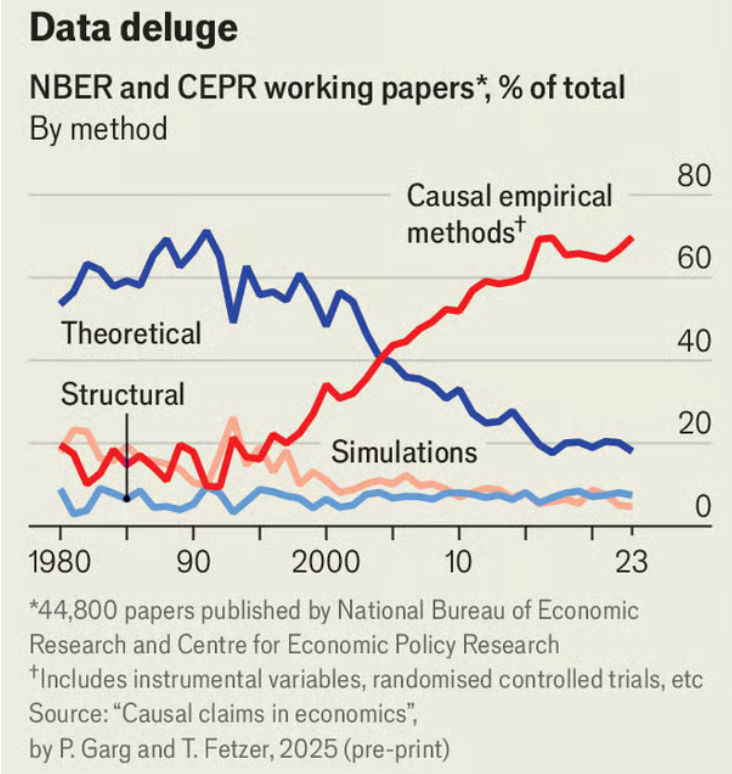
\includegraphics[scale=0.4]{./lecture_includes/causal_claims}
	\end{figure}

\end{frame}

\begin{frame}{Diff-in-Diff Over Time}

	\begin{figure}
	\caption{Currie, et al. (2020)}
	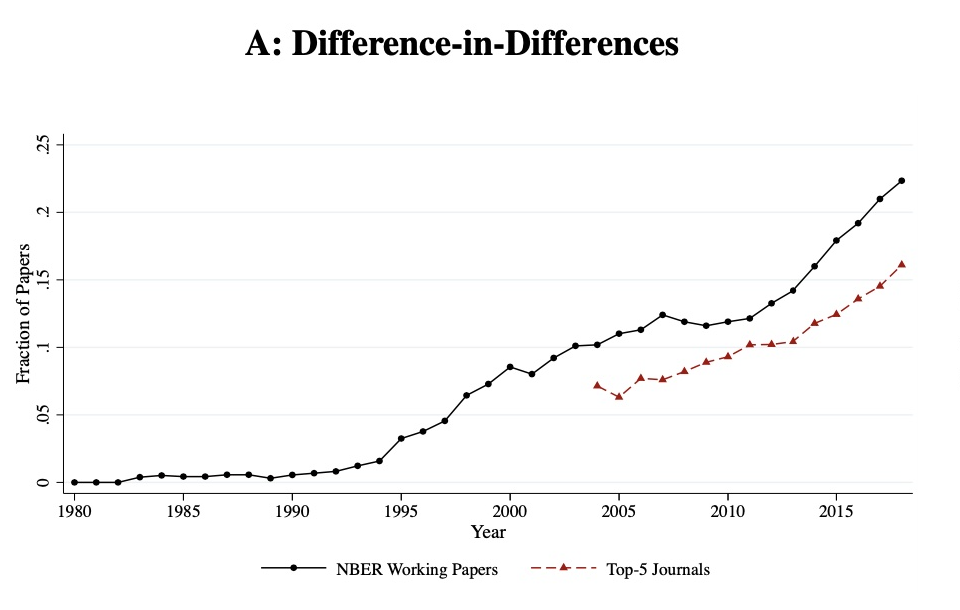
\includegraphics[scale=0.25]{./lecture_includes/currie_did.png}
	\end{figure}

\end{frame}

\begin{frame}{Diff-in-Diff Compared to Others Over Time}

	\begin{figure}
	\caption{Garg and Fetzer (2025)}
	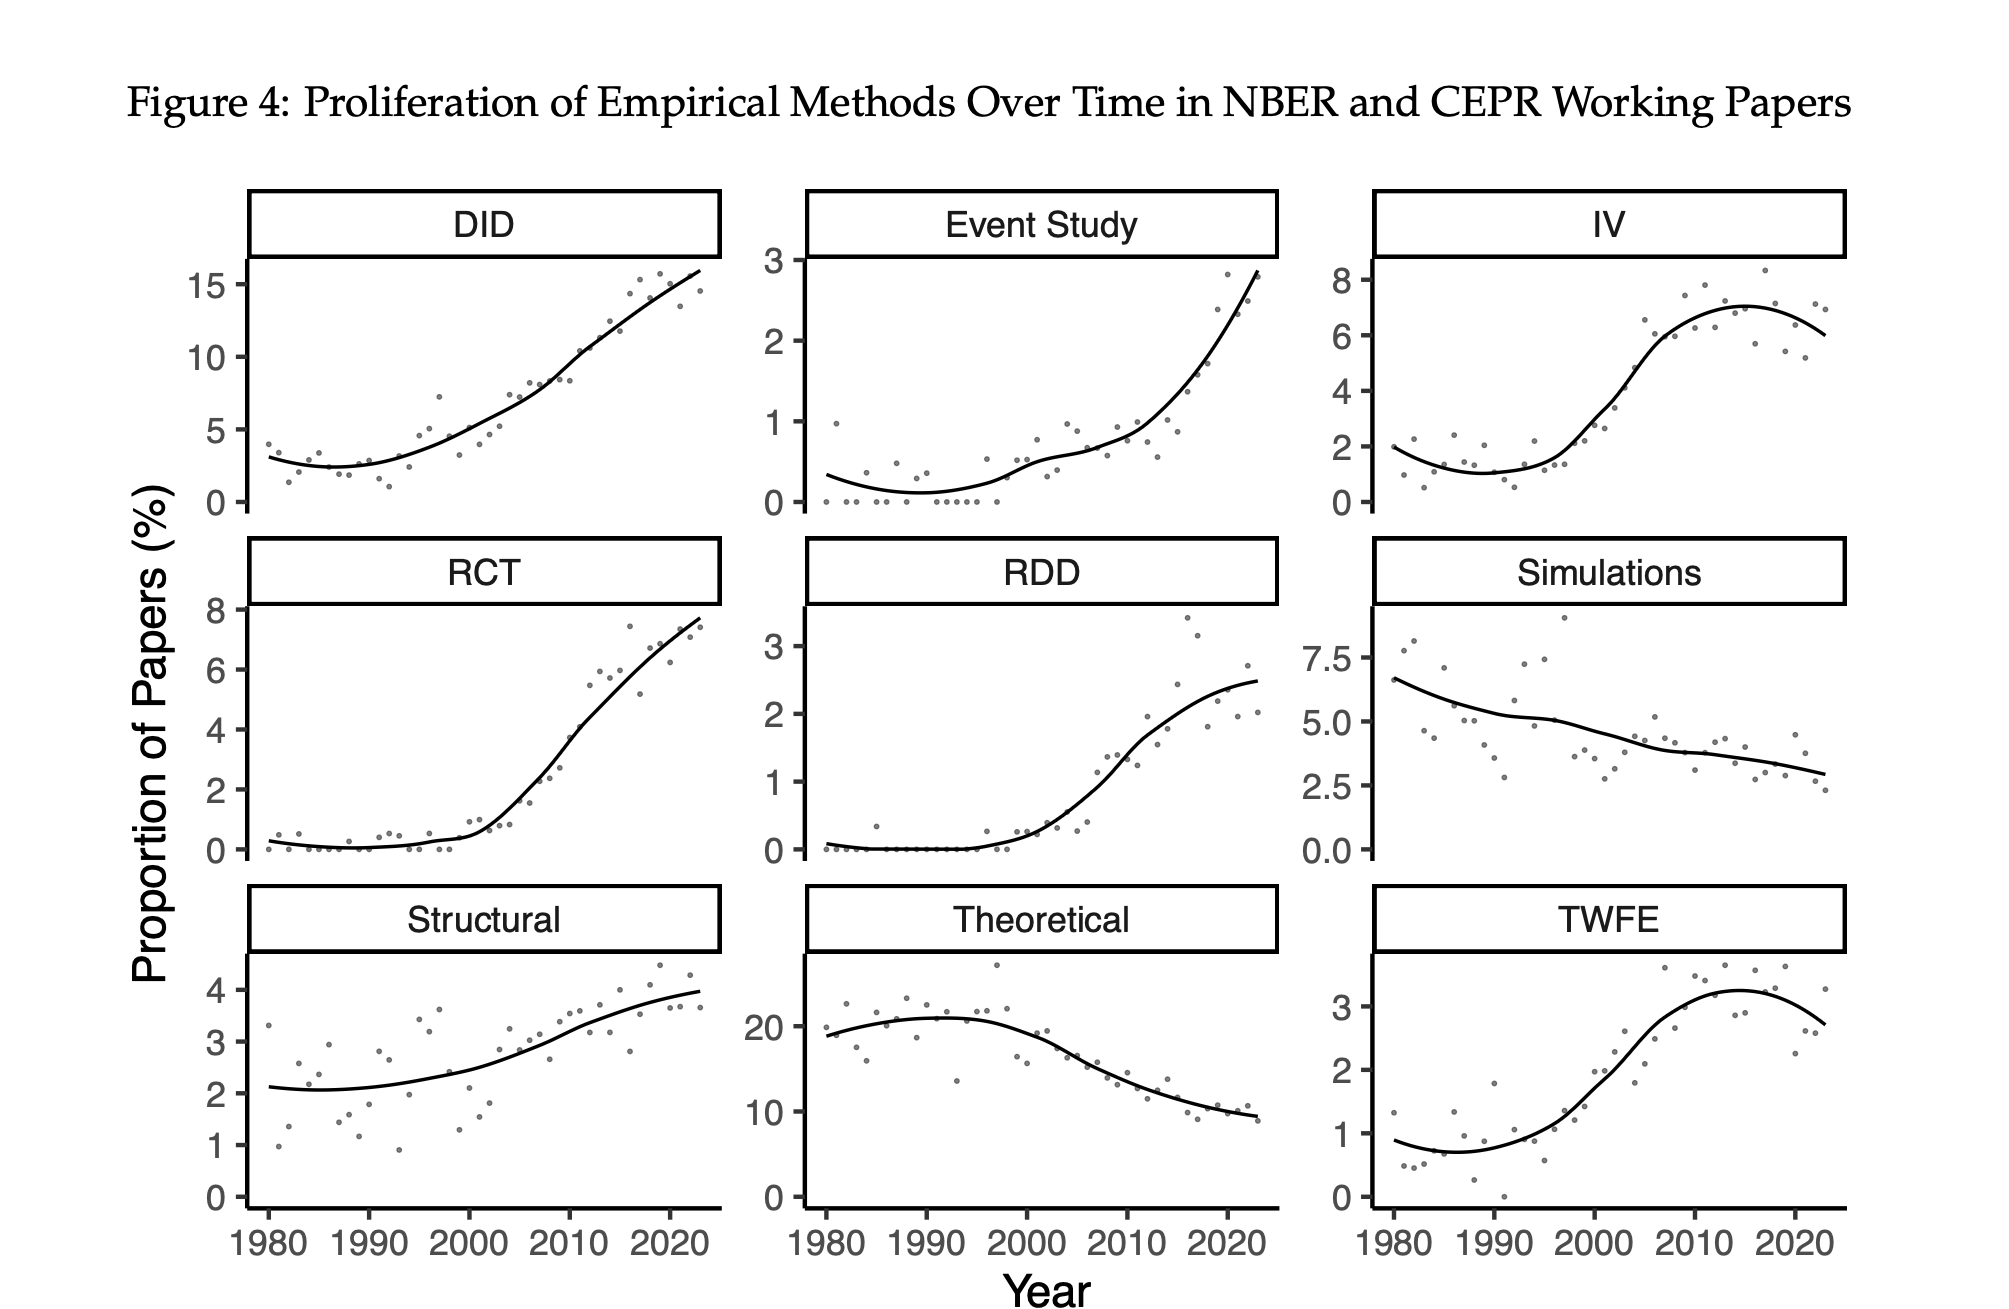
\includegraphics[scale=0.25]{./lecture_includes/did_growth1}
	\end{figure}

\end{frame}





\begin{frame}{Diff-in-Diff in the Cross-Section by Field}

	\begin{figure}
	\caption{Garg and Fetzer (2025)}
	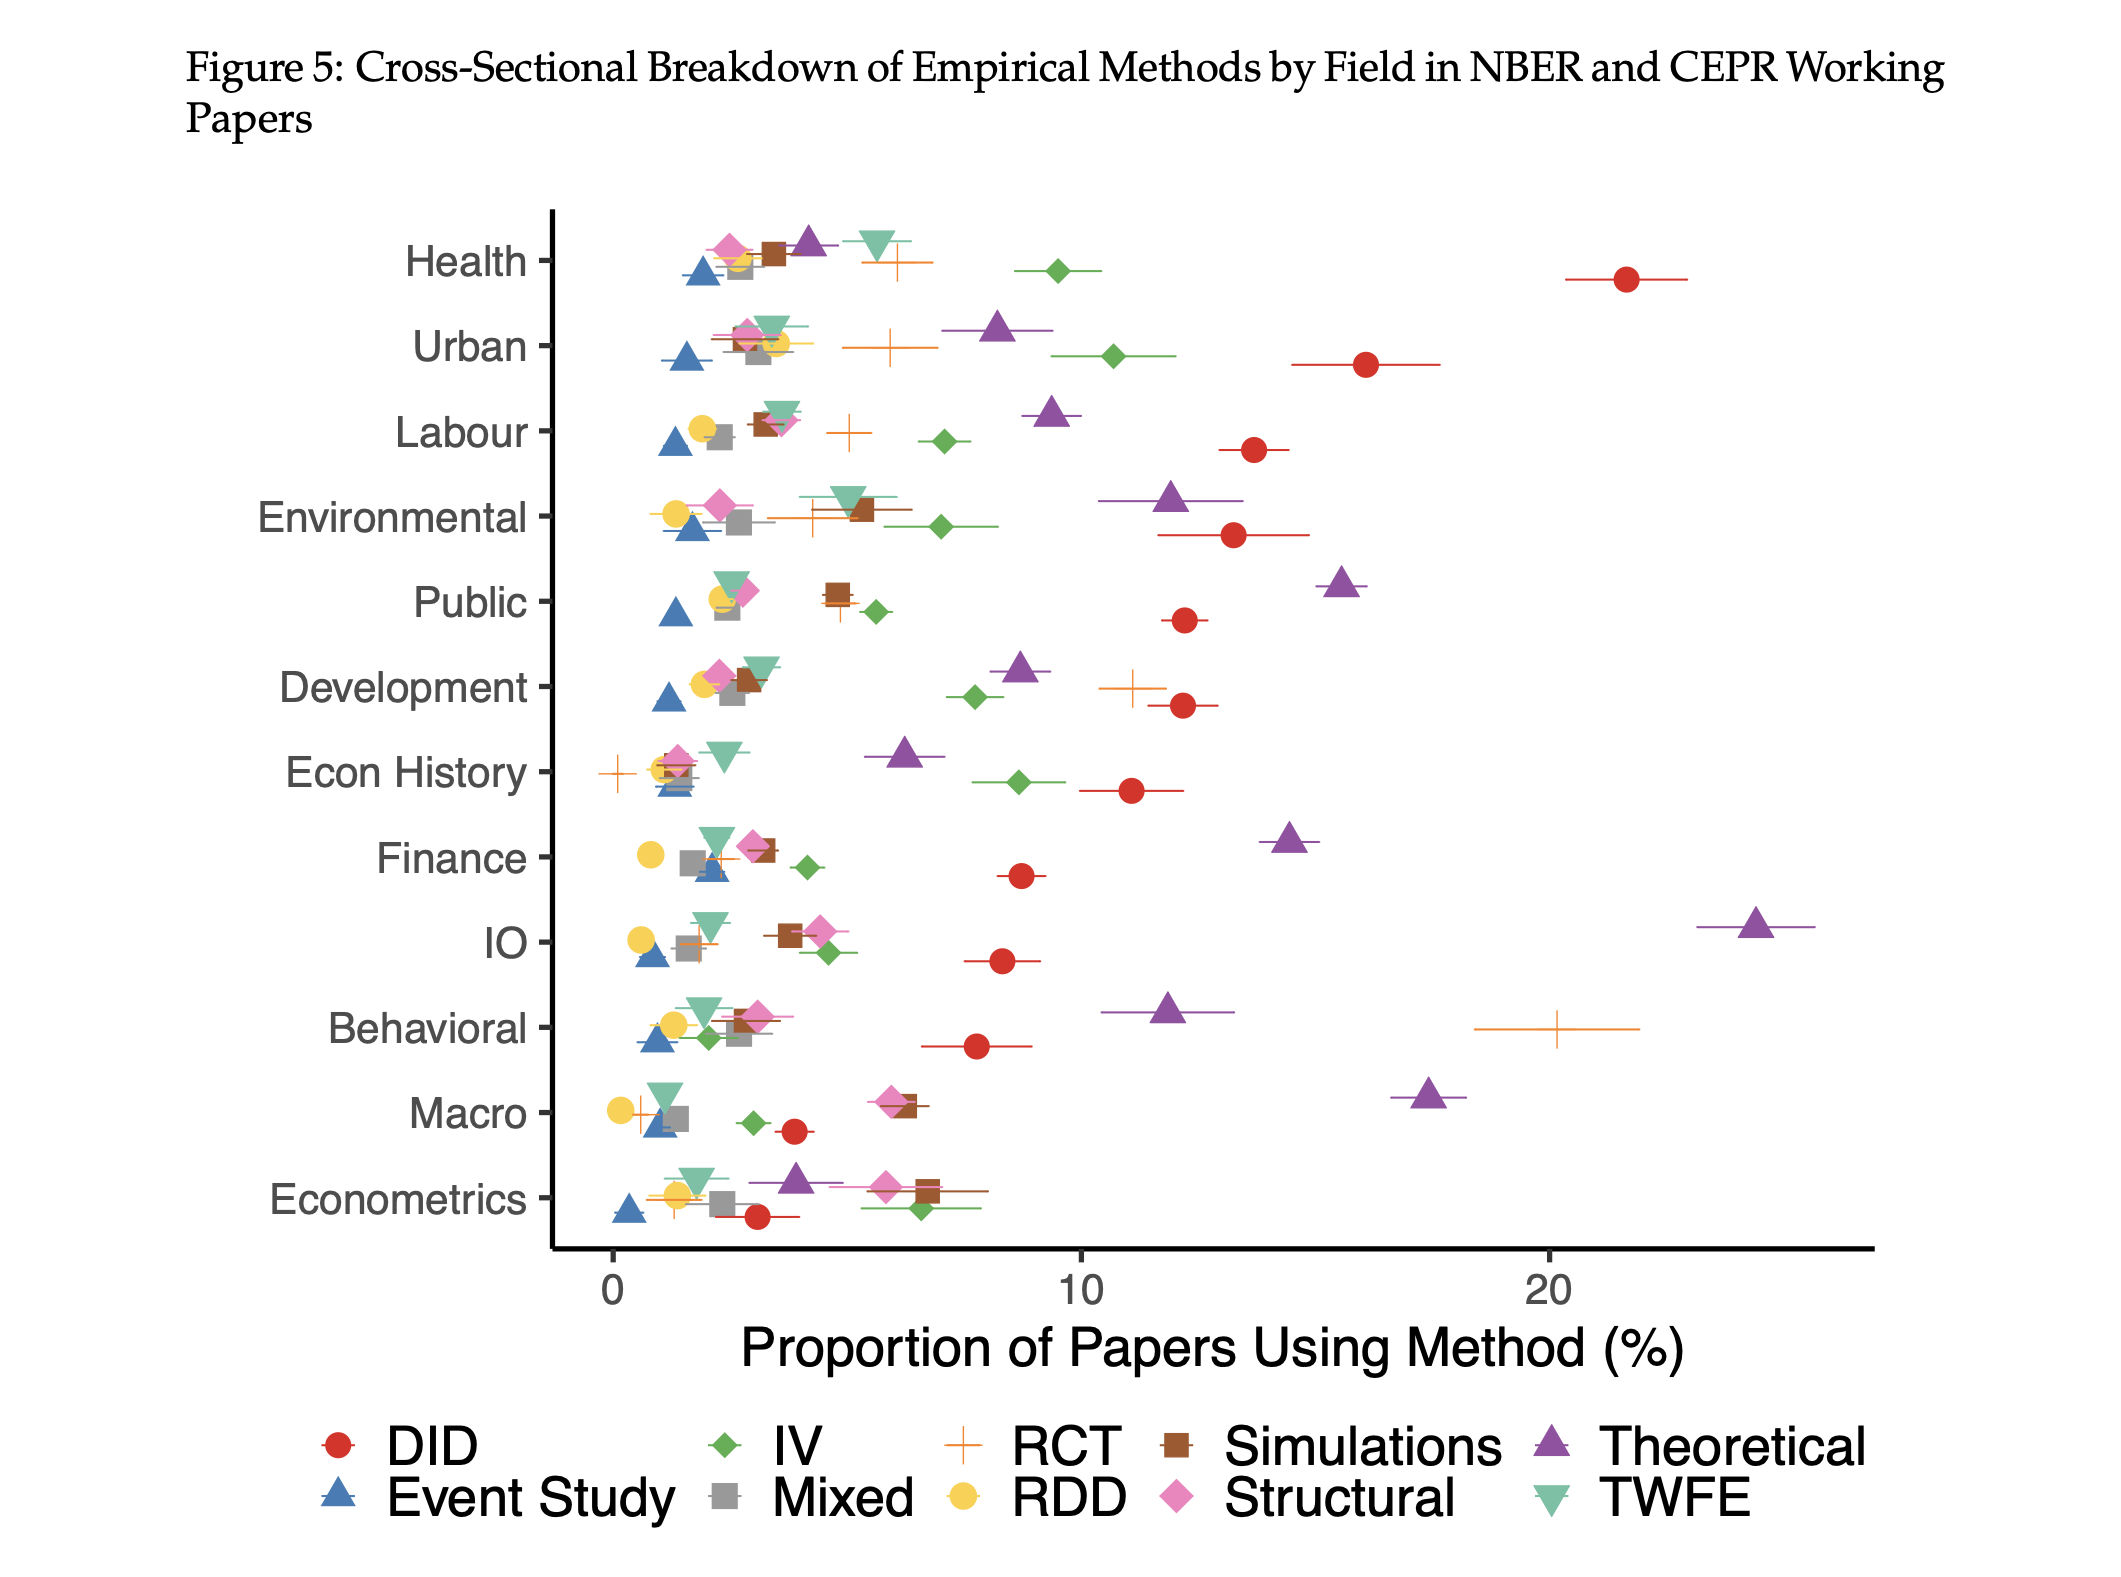
\includegraphics[scale=0.25]{./lecture_includes/did_growth2}
	\end{figure}

\end{frame}



\begin{frame}{Diff-in-Diff Over Time by Field}

	\begin{figure}
	\caption{Goldsmith-Pinkham (2024)}
	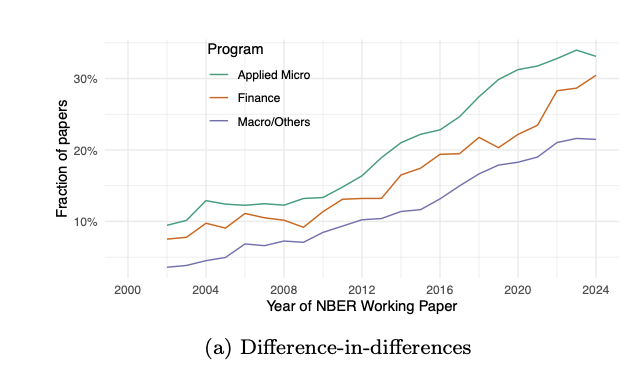
\includegraphics[scale=0.75]{./lecture_includes/paul_did}
	\end{figure}

\end{frame}







\subsection{Origins of diff-in-diff in public health}


\begin{frame}{Ignaz Semmelweis and washing hands}

\begin{itemize}
\item Early 1820s, Vienna passed legislation requiring that if a pregnant women giving birth went to a public hospital (free care), then depending on the day of week and time of day, she would be routed to either the midwife wing or the physician wing (most likely resulting in random assignment)
\item But by the 1840s, Ignaz Semmelweis noticed that pregnant women died after delivery in the (male) wing at a rate of 13-18\%, but only 3\% in the (female) midwife wing -- cause was puerperal or “childbed” fever
\item Somehow this was also we known -- women would give birth in the street rather than go to the physician if they were unlucky enough to have their water break on the wrong day and time
\end{itemize}

\end{frame}

\begin{frame}{Ignaz Semmelweis and washing hands}

\begin{itemize}
\item Ignaz Semmelweis conjectures after a lot of observation that the cause is the teaching faculty teaching anatomy using cadavers and then delivering babies \emph{without washing hands}
\item New training happens to one but not the other and Semmelweis thinks the mortality is caused by working with cadavers
\item Convinced the hospital to have physicians wash their hands in chlorine but not the midwives, creating a type of difference-in-differences design
\end{itemize}

\end{frame}

\begin{frame}{Semmelweis diff-in-diff evidence}

	\begin{figure}
	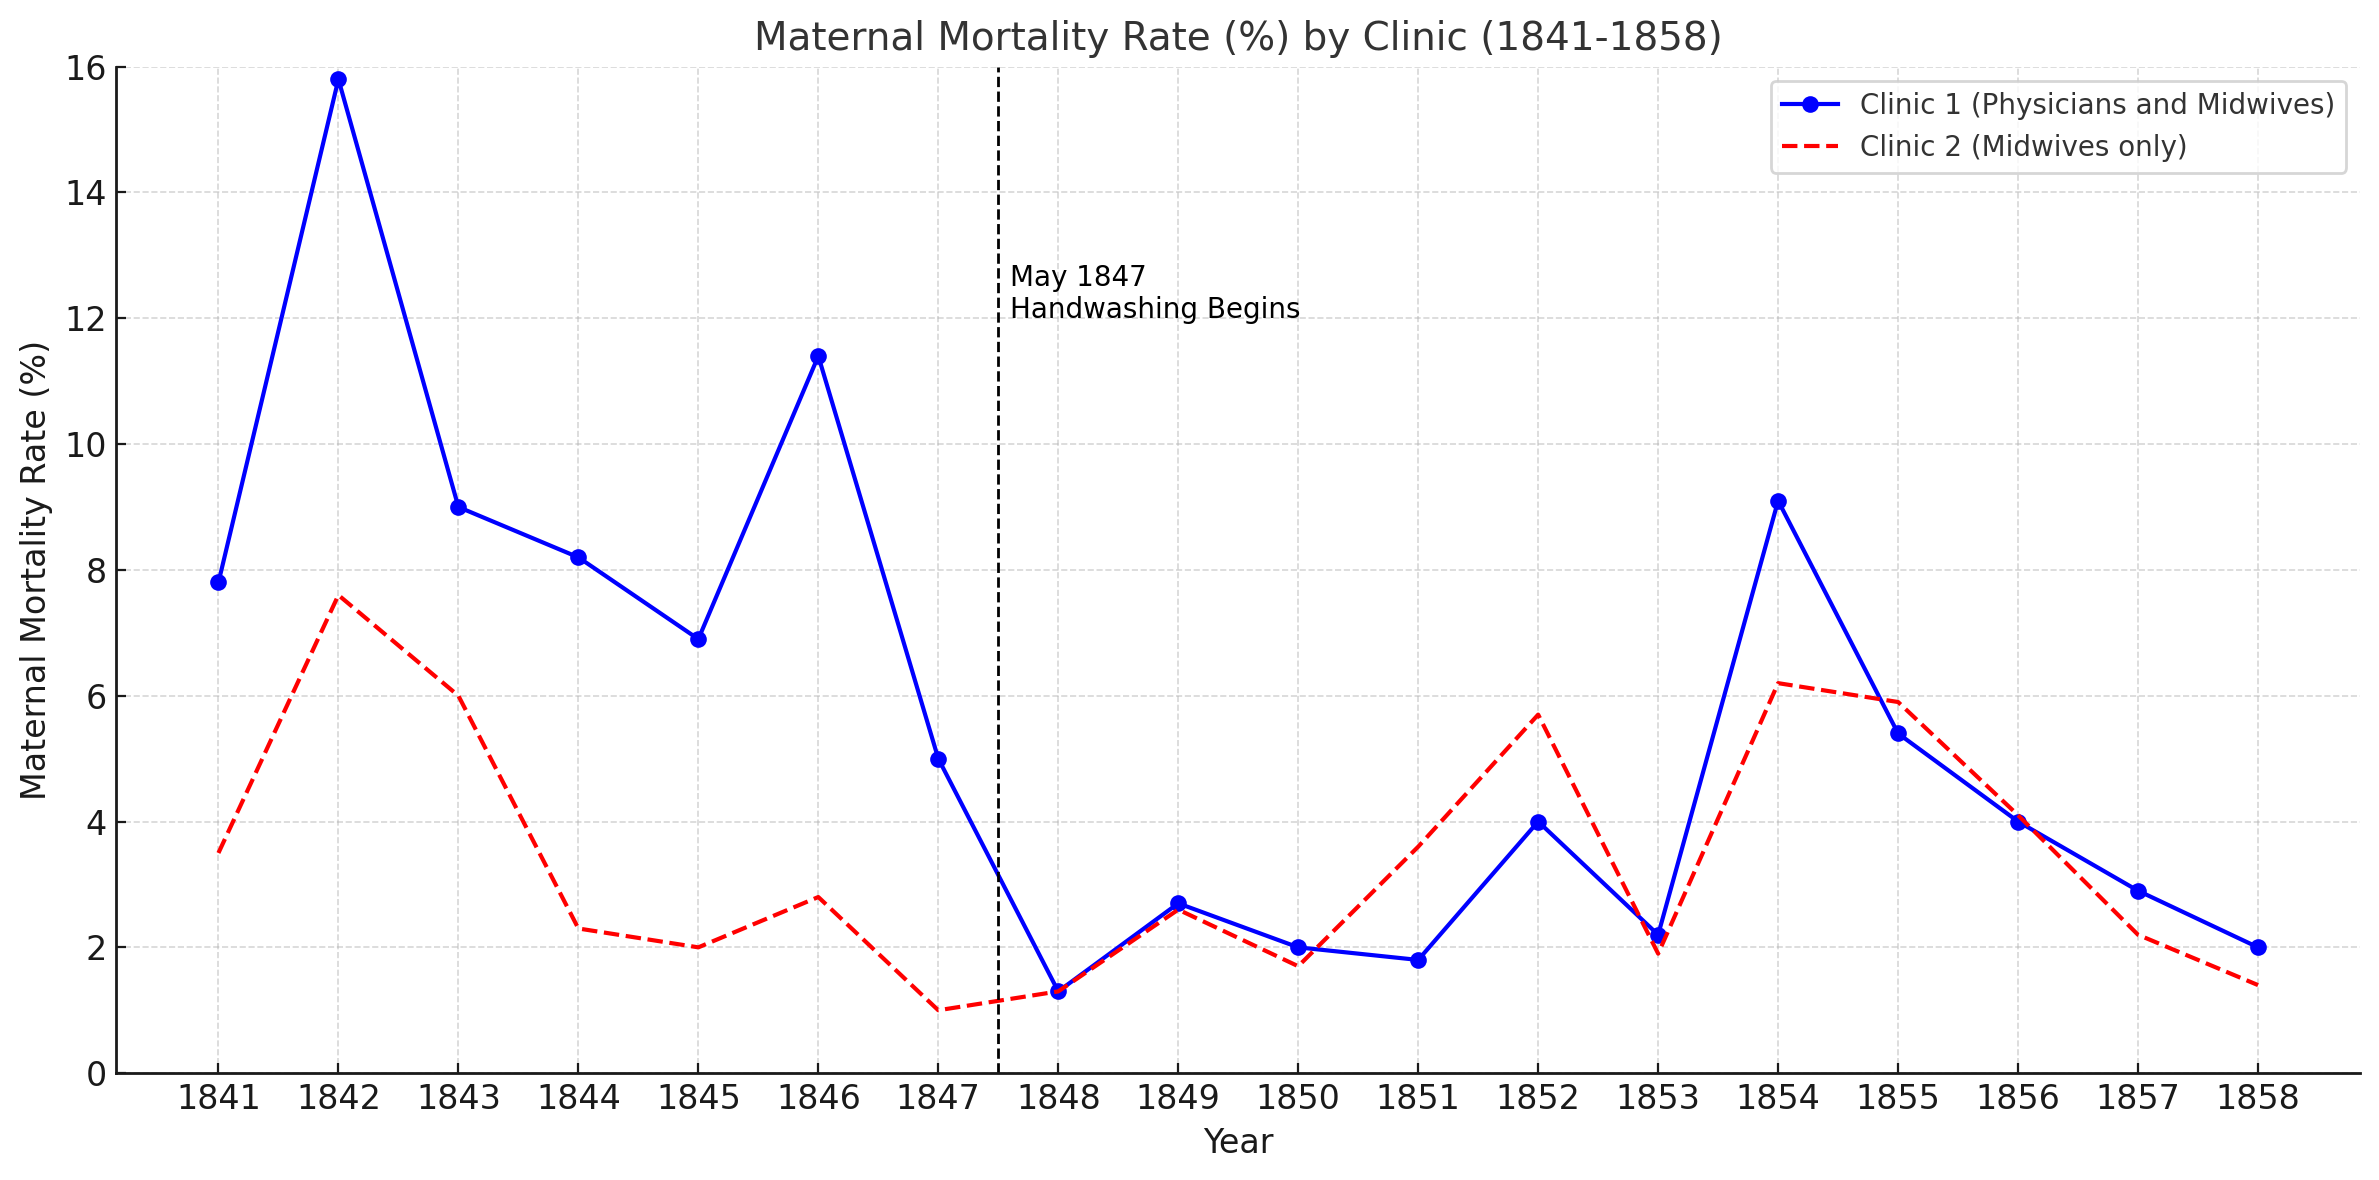
\includegraphics[scale=0.4]{./lecture_includes/semmelweis_graphic.png}
	\end{figure}


\end{frame}

\begin{frame}{Evidence Rejected}

\begin{itemize}

\item Diff-in-diff evidence was rejected by Semmelweis' superiors claiming it was the hospital's new ventilation system
\item Dominant theory of disease spread was caused by "odors" or miasma or "humors"
\item Semmelweis began showing signs of irritability, perhaps onset of dementia, became publicly abusive, was committed to a mental hospital and within two weeks died from wounds he received while in residence
\item Despite the strength of evidence, difference-in-differences was rejected -- a theme we will see continue

\end{itemize}

\end{frame}






\begin{frame}{John Snow and cholera}

\begin{itemize}
\item Three major waves of cholera in the early to mid 1800s in London, largely thought to be spread by miasma (``dirty air'')
\item John Snow believed cholera was spread through the Thames water supply through an invisible creature that entered the body through food and drink, caused the body to expel water, placing the creature back in the Thames and causing epidemic waves
\item London passes ordinance requiring water utility companies to move inlet pipe further up the Thames, above the city center, but not everyone complies
\item Natural experiment: Lambeth water company moves its pipe between 1849 and 1854; Southwark and Vauxhall water company delayed
\end{itemize}

\end{frame}


\begin{frame}

	\begin{figure}
	\caption{Two water utility companies in London 1854}
	\includegraphics[scale=0.225]{./lecture_includes/lambeth.png}
	\end{figure}


\end{frame}



\begin{frame}{Difference-in-differences}

\begin{table}\centering
\scriptsize
		\caption{Lambeth and Southwark and Vauxhall, 1849 and 1854}
		\begin{center}
		\begin{tabular}{lll|lc}
		\toprule
		\multicolumn{1}{l}{\textbf{Companies}}&
		\multicolumn{1}{c}{\textbf{Time}}&
		\multicolumn{1}{c}{\textbf{Outcome}}&
		\multicolumn{1}{c}{$D_1$}&
		\multicolumn{1}{c}{$D_2$}\\
		\midrule
		Lambeth & Before & $Y=L$ \\
		& After & $Y=L + L_t + D$ & $\textcolor{red}{L_t}+D$\\
		\midrule
		& & & & $D + (\textcolor{red}{L_t}- SV_t)$ \\
		\midrule
		Southwark and Vauxhall & Before & $Y=SV$ \\
		& After & $Y=SV + SV_t$ & $SV_t$\\
		\bottomrule
		\end{tabular}
		\end{center}
	\end{table}

\begin{eqnarray*}
\widehat{\delta}_{did} = D + (\textcolor{red}{L_t}- SV_t)
\end{eqnarray*}This method yields an unbiased estimate of D if $\textcolor{red}{L_t} = SV_t$, but note that $\textcolor{red}{L_t}$ is a counterfactual trend and therefore not known

\end{frame}

\begin{frame}{Will You Be Able to Spot the Problem by Friday?}

\begin{itemize}
\item Both of these have the correct \emph{calculation}
\item \emph{But} one of them is robust to unrestricted heterogenous treatment effects but \emph{one of them is not}
\item \textbf{Which one is robust and which one is not!?}
\item If you can answer this correctly for the exam, you will get 5 points extra credit. 
\end{itemize}

\end{frame}

\section{Diff-in-Diff Fundamentals}

\subsection{$\mathbf{2 \times 2}$ Equation}

\begin{frame}{DiD equation is the 2x2}

\begin{itemize}
\item The building block of diff-in-diff calculations is the $\mathbf{2 \times 2}$ 
\item Two groups, two time periods, four averages, three subtractions ("four averages and three subtractions")
\item Often called the $2 \times 2$ for that reason (Goodman-Bacon 2021)

\begin{eqnarray*}
\widehat{\delta} = \bigg ( E[Y_k|Post] - E[Y_k|Pre] \bigg ) - \bigg ( E[Y_U | Post ] - E[ Y_U | Pre] \bigg) \\
\end{eqnarray*}$k$ are the people in the job training program, $U$ are the untreated people not in the program, $Post$ is after the trainees took the class, $Pre$ is the period just before they took the class, and $E[y]$ is mean earnings.
\item See \url{https://docs.google.com/spreadsheets/d/1onabpc14JdrGo6NFv0zCWo-nuWDLLV2L1qNogDT9SBw/edit?usp=sharing}
\end{itemize}

\end{frame}



\begin{frame}{Why do Diff-in-Diff}

\begin{itemize}
\item Appeal of diff-in-diff has \emph{always} been its simplicity, its transparency, and its ease of conveying analysis to an audience
	\begin{itemize}
	\item Giovanni Mastrobuoni graduated from Princeton University in 2006 and studied with a famous labor economist named Orley Ashenfelter
	\item Orley invented the term "difference-in-differences" used it in the 1970s to explain regressions with fixed effects to US Bureaucrats
	\end{itemize}
\item Diff-in-diff is four averages and three subtractions and everyone knows what those are
$$\widehat{\textcolor{blue}{\delta}} = \bigg ( \overline{y}_k^{post(k)} - \overline{y}_k^{pre(k)} \bigg ) - \bigg ( \overline{y}_U^{post(k)} - \overline{y}_U^{pre(k)} \bigg ) $$
\item But $\widehat{\delta}$ is just the OLS coefficient in this regression:
$$Y_{ist} = \alpha_0 + \alpha_1 Treat_{is} + \alpha_2 Post_{t} + \textcolor{blue}{\delta} (Treat_{is} \times Post_t) + \varepsilon_{ist} $$
\end{itemize}

\end{frame}


\begin{frame}{Data example}

\begin{itemize}
\item Medicaid is a US policy for the poor -- provides access to healthcare to the poor -- and it's been a research question whether it has any effect on mortality
	\begin{itemize}
	\item Finkelstein, et al. (2012) found no effect on mortality from RCT, but it was probably underpowered to find small effects
	\item Borgschulte and Vogler (2020) used county level publicly available mortality data and found evidence that it did
	\item Miller, Johnson and Wherry (2022) used linked administrative data and also found it did
	\end{itemize}
\item Let's review the Borgschulte and Vogler (2020) approach

\end{itemize}

\end{frame}

\begin{frame}{Simple 2x2 DD}

\begin{figure}
    \centering
    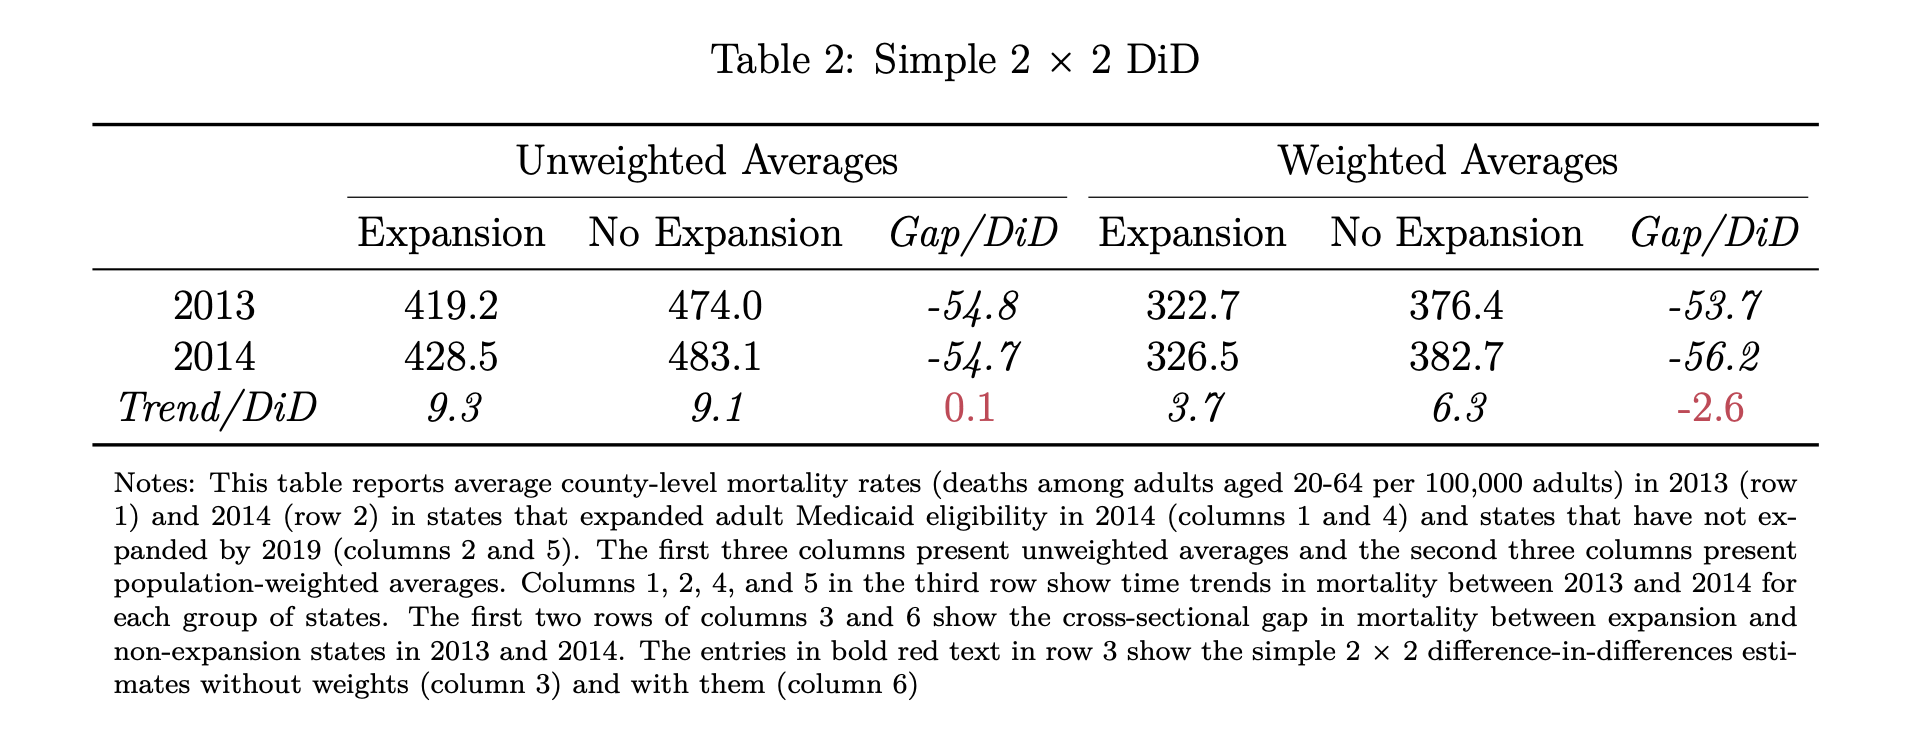
\includegraphics[height=0.5\textheight]{./lecture_includes/simple2x2.png}
\end{figure}




\end{frame}

\begin{frame}{Minimum wages}

\begin{itemize}
\item Card and Krueger (1994) have a famous study estimating causal effect of minimum wages on employment
\item  New Jersey raises its minimum wage in April 1992 (between February and November) but neighboring Pennsylvania does not
\item Using DiD, they do not find a negative effect of the minimum wage on employment leading to complex reactions from economists
\item Orley's describes his understanding of people's reaction to the paper.  \\ \url{https://youtu.be/MOtbuRX4eyQ?t=1882}
\end{itemize}

\end{frame}

\begin{frame}
	\begin{figure}
	
\includegraphics[scale=0.5]{./lecture_includes/minwage_whore}
	\end{figure}
\end{frame}


\begin{frame}{Reaction to the paper}


Lots of anecdotes in this interview with Card, but here are just two.  First, Card and Krueger received a lot of personal hostility from their peers (1:07 to 1:10)

\bigskip

\url{https://youtu.be/1soLdywFb_Q?si=laAVYf_E2KBZKywG&t=4020}

\bigskip

Later Card says Sherwin Rosen accused them of having an agenda.  But the worst is what happens to Alan Krueger maybe (1:16 to 1:17)

\bigskip

\url{https://youtu.be/1soLdywFb_Q?si=jsb8h50ZosGDnKrv&t=4556}




\end{frame}

\begin{frame}{Card on that study}

\begin{quote}
``I’ve subsequently stayed away from the minimum wage literature for a number of reasons. First, it cost me a lot of friends. People that I had known for many years, for instance, some of the ones I met at my first job at the University of Chicago, became very angry or disappointed. They thought that in publishing our work we were being traitors to the cause of economics as a whole.''
\end{quote}


\end{frame}



\begin{frame}{OLS specification of the DiD equation}
	
	\begin{itemize}
	\item The correctly specified OLS regression is an interaction with time and group fixed effects:$$Y_{its} = \alpha + \gamma NJ_s + \lambda d_t + \delta (NJ \times d)_{st} + \varepsilon_{its}$$
		\begin{itemize}
		\item NJ is a dummy equal to 1 if the observation is from NJ
		\item d is a dummy equal to 1 if the observation is from November (the post period)
		\end{itemize}
	\item This equation takes the following values
		\begin{itemize}
		\item PA Pre: $\alpha$
		\item PA Post: $\alpha + \lambda$
		\item NJ Pre: $\alpha + \gamma$
		\item NJ Post: $\alpha + \gamma + \lambda + \delta$
		\end{itemize}
	\item DiD equation: (NJ Post - NJ Pre) - (PA Post - PA Pre) $= \delta$
	\end{itemize}
\end{frame}




\begin{frame}[plain]
	$$Y_{ist} = \alpha + \gamma NJ_s + \lambda d_t + \delta(NJ\times d)_{st} + \varepsilon_{ist}$$
	\begin{figure}
	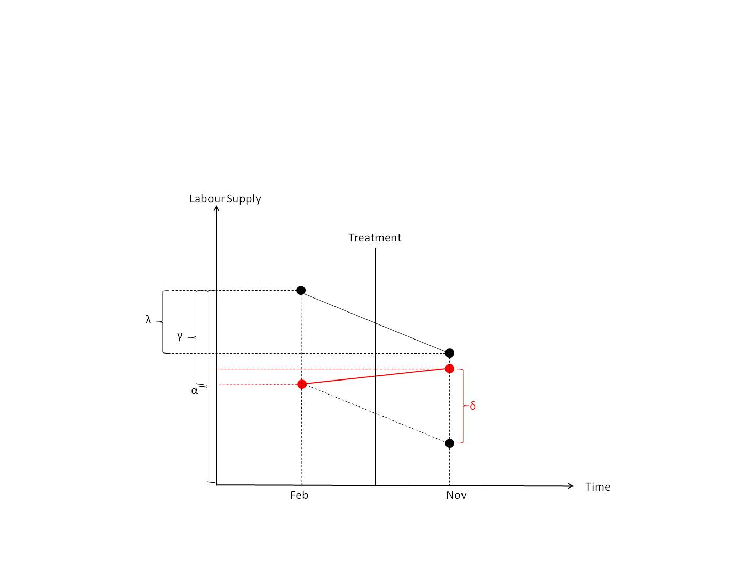
\includegraphics[scale=0.90]{./lecture_includes/waldinger_dd_5.pdf}
	\end{figure}
\end{frame}


\begin{frame}[plain]
	$$Y_{ist} = \alpha + \gamma NJ_s + \lambda d_t + \delta(NJ\times d)_{st} + \varepsilon_{ist}$$
	\begin{figure}
	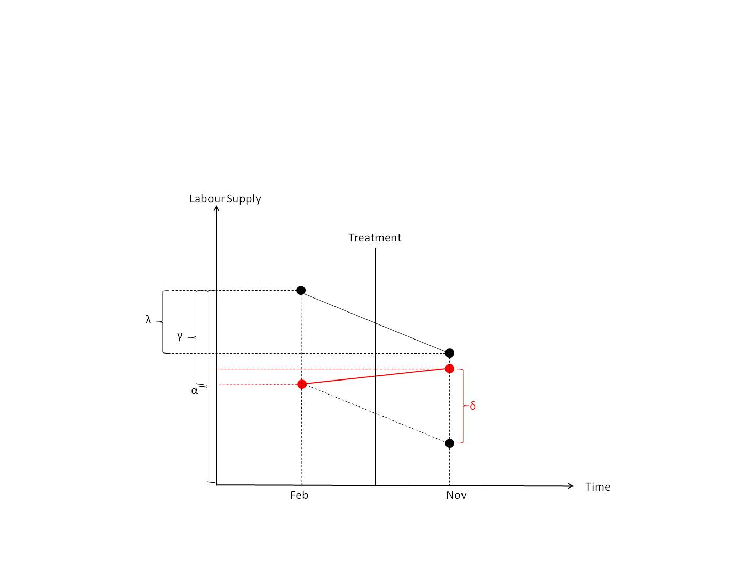
\includegraphics[scale=0.90]{./lecture_includes/waldinger_dd_5.pdf}
	\end{figure}

Notice how OLS is ``imputing'' $E[Y^0|D=1,Post]$ for the treatment group in the post period? It is only ``correct'', though, if parallel trends is a good approximation

\end{frame}





\begin{frame}{Three Regressions}

\begin{itemize}
\item Three regression specifications give you those exact same numbers
	\begin{enumerate}
	\item Regress mortality onto treatment dummy, post dummy and interaction (no fixed effects)
	\item Regress mortality onto interaction with county and year fixed effects (but no constant)
	\item Regress long difference (i.e., post value minus pre) onto a treatment dummy
	\end{enumerate}
\item Those are all numerically identical to "four averages and three subtractions"
\end{itemize}

\end{frame}

\begin{frame}

\begin{figure}
    \centering
    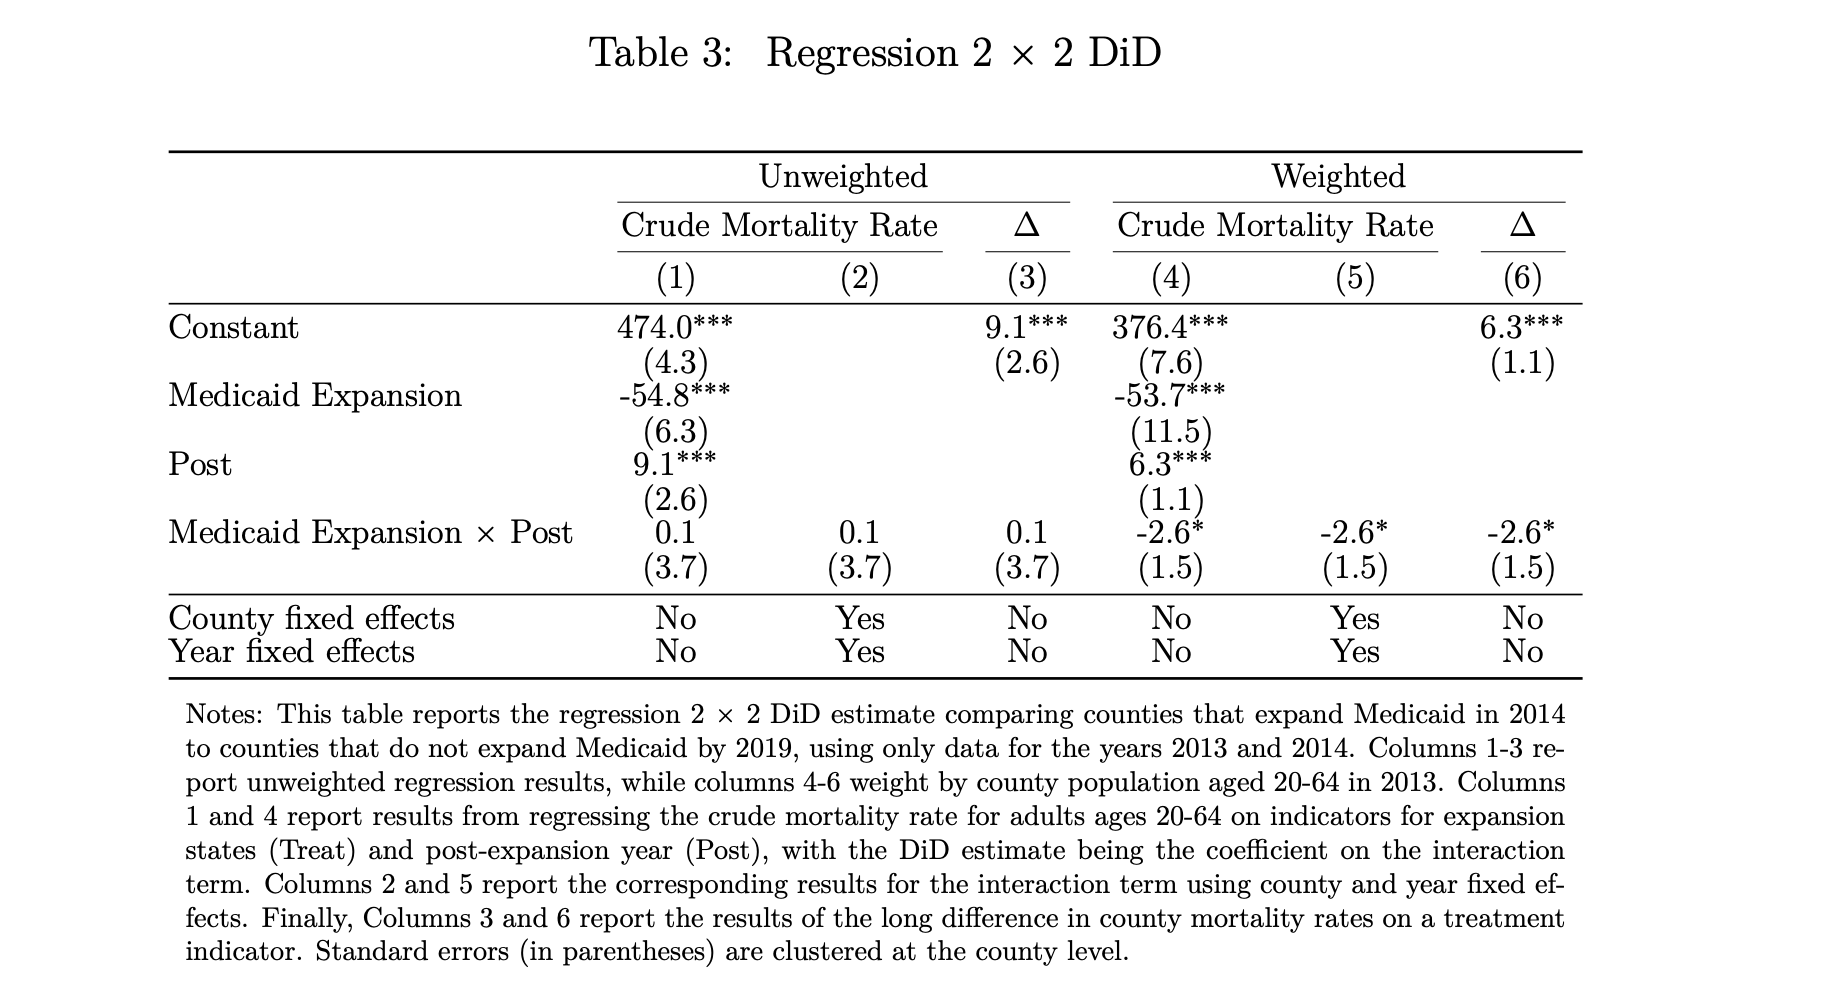
\includegraphics[height=0.7\textheight]{./lecture_includes/regression2x2.png}
\end{figure}

\end{frame}



\begin{frame}{Equivalence}

\begin{itemize}

\item Equivalence between calculating these 2x2s by hand or with a regression has appealing features
\item Regressions are simple to run, and they do the averaging behind the scenes
\item They also allow us to use statistical inference tools from OLS like clustering decisions
\item Bertrand, Duflo and Mullainathan (2004) show that conventional standard errors will often severely understate the standard deviation of the estimators and propose clustering standard errors at the aggregate unit level of treatment
\item Please open \texttt{equivalence.do} and \texttt{equivalence.R} in ./Example-Code
\end{itemize}

\end{frame}






\subsection{Average Treatment Effect on the Treated}



\begin{frame}{Deriving identification assumptions}

\begin{itemize}

\item Diff-in-diff is two things
	\begin{enumerate}
	\item It's \textcolor{blue}{always} a calculation (i.e., four averages)
	\item It \textcolor{red}{sometimes} has a causal interpretation
	\end{enumerate}
\item I'm going to walk us through two main assumptions using potential outcomes and algebra
\item Then we will look at what happens when our control group has been treated (not an assumption, more like a promise)
\end{itemize}

\end{frame}







\begin{frame}{Potential outcomes notation}

	\begin{itemize}
	\item Let the treatment be a binary variable: $$D_{i,t} =\begin{cases} 1 \text{ if in job training program $t$} \\ 0 \text{ if not in job training program at time $t$} \end{cases}$$where $i$ indexes an individual observation, such as a person

	\end{itemize}
\end{frame}

\begin{frame}{Potential outcomes notation}

	\begin{itemize}

	\item Potential outcomes: $$Y_{i,t}^j =\begin{cases} 1 \text{: wages at time $t$ if trained} \\ 0 \text{: wages at time $t$ if not trained} \end{cases}$$where $j$ indexes a state of the world where the treatment happened or did not happen

	\end{itemize}
\end{frame}



\begin{frame}{Treatment effect definitions}


	\begin{block}{Individual treatment effect}
	    The individual treatment effect,  $\delta_i$, equals $Y_i^1-Y_i^0$
	\end{block}

Missing data problem:  No data on the counterfactual

\end{frame}


\begin{frame}{Average Treatment Effects for the Treated Subpopulation}
	\begin{block}{Average Treatment Effect on the Treated (ATT)}
	The average treatment effect on the treatment group is equal to the average treatment effect conditional on being a treatment group member:
		\begin{eqnarray*}
		E[\delta|D=1]&=&E[Y^1-Y^0|D=1] \nonumber \\
		&=&E[Y^1|D=1]-\textcolor{red}{E[Y^0|D=1]}
		\end{eqnarray*}
	\end{block}

	\bigskip

It's the average causal effect but only for the people exposed to some intervention; notice we can't calculate it, also, because we are missing the red term


\end{frame}

\begin{frame}{ATT vs ATE}

\begin{itemize}
\item Potential outcomes is subtle and easily people are overconfident about its interpretation (probably because counterfactuals are seemingly easy to understand)
\item Let's look at the "Potential Outcomes" tab at our Diff-in-Diff Worksheet; fill out all the instructions 
\item \url{https://docs.google.com/spreadsheets/d/1onabpc14JdrGo6NFv0zCWo-nuWDLLV2L1qNogDT9SBw/edit?usp=sharing}
\end{itemize}

\end{frame}




\subsection{Core Diff-in-Diff Assumptions}

\begin{frame}{Causal Parameters}

\begin{itemize}
\item Causal parameters have three ingredients:
	\begin{enumerate}
	\item Potential outcome notation and treatment effects (i.e., $\delta_i = Y^1_i - Y^0_i$)
	\item Populations of units
	\item Averages and weights (though there are alternatives)
	\end{enumerate}
\item There are oftentimes more than one causal parameter, and when you choose among them, that is called your \textbf{target parameter}
\end{itemize}

\end{frame}

\begin{frame}{Identification vs Estimation}

\begin{itemize}
\item Very common for someone to write down:

$$ Y_{it} = \alpha + \beta D_{it} + \tau_t + \sigma_s + \varepsilon_{it}$$and say that $\beta$ is their causal parameter -- it is not

\item We start by distinguishing between the parameter we are attempting to identify and the manner in which we will estimate it
\item Identification requires first stating explicitly our goal expressed using potential outcomes
\item But often people skip this step and go directly to regressions which creates confusion and misinterpretation

\end{itemize}

\end{frame}



\begin{frame}{Start with simple $\mathbf{2 \times 2}$ equation}

\begin{eqnarray*}
\widehat{\delta} &=& \bigg ( \underbrace{E[Y_k|Post] - E[Y_k|Pre] \bigg ) - \bigg ( E[Y_U | Post ] - E[ Y_U | Pre]}_{\mathclap{\text{$\mathbf{2 \times 2}$ equation}}} \bigg)  
\end{eqnarray*}

\bigskip

Recall this can be calculated manually or using one of three regression specifications -- they are all the simple $\mathbf{2 \times 2}$. 


\end{frame}



\begin{frame}{Replace realized outcome with potential outcomes}

\begin{eqnarray*}
\widehat{\delta} &=& \bigg ( \underbrace{E[Y^1_k|Post] - E[Y^0_k|Pre] \bigg ) - \bigg ( E[Y^0_U | Post ] - E[ Y^0_U | Pre]}_{\mathclap{\text{Switching equation}}} \bigg) 
\end{eqnarray*}

\bigskip

Notice we replaced each $Y$ term with its potential outcome, $(Y^1, Y^0)$, depending on whether that group in that period was or was not treated. 

\bigskip

Nothing in the $\mathbf{2 \times 2}$ is a \emph{causal parameter} as no treatment effects appear


\end{frame}

\begin{frame}{Replace with potential outcomes and add a zero}

\begin{eqnarray*}
\widehat{\delta} &=& \bigg ( \underbrace{E[Y^1_k|Post] - E[Y^0_k|Pre] \bigg ) - \bigg ( E[Y^0_U | Post ] - E[ Y^0_U | Pre]}_{\mathclap{\text{Switching equation}}} \bigg)  \\
&&+ \underbrace{\textcolor{red}{E[Y_k^0 |Post] - E[Y^0_k | Post]}}_{\mathclap{\text{Adding zero}}}
\end{eqnarray*}


\end{frame}


\begin{frame}{Non-parallel trends bias term}

\begin{eqnarray*}
\widehat{\delta} &=& \underbrace{E[Y^1_k | Post] - \textcolor{red}{E[Y^0_k | Post]}}_{\mathclap{\text{ATT}}} \\
&& + \bigg [  \underbrace{\textcolor{red}{E[Y^0_k | Post]} - E[Y^0_k | Pre] \bigg ] - \bigg [ E[Y^0_U | Post] - E[Y_U^0 | Pre] }_{\mathclap{\text{Non-parallel trends bias in 2x2 case}}} \bigg ]
\end{eqnarray*}

\bigskip

The $\mathbf{2 \times 2}$ equals the sum of 1) a causal parameter plus 2) a bias term called the non-parallel trends bias term and 3) notice this is the $\mathbf{2 \times 2}$ not the $\mathbf{2 \times T}$ (e.g., event study)


\end{frame}

\begin{frame}{Identification through parallel trends}


	\begin{block}{Parallel trends}
	Assume two groups, treated and comparison group, then we define parallel trends as:	 $$\textcolor{red}{E(}\textcolor{red}{\Delta Y^0_k)} = E(\Delta Y^0_U)$$
	\end{block}

\textbf{In words}: ``The \textcolor{red}{evolution of earnings for our trainees \emph{had they not trained}} is the same as the evolution of mean earnings for non-trainees''.

\bigskip

It's in \textcolor{red}{red} because parallel trends is untestable and critically important to estimation of the ATT using any method, OLS or ``four averages and three subtractions''

\end{frame}

\begin{frame}{Don't Need More Than Two Periods}

\begin{itemize}

\item Notice that diff-in-diff identifies the ATT \emph{with only} two time periods
\item Diff-in-diff does not "need" a long pre-treatment time series (unlike synthetic control which does) -- two periods and two groups is enough
\item But there is another assumption aside from parallel trends we want to learn

\end{itemize}

\end{frame}

\begin{frame}{No Anticipation}

\begin{itemize}
\item First interpretation of No Anticipation (NA) is this:
	\begin{eqnarray*}
	Y_{i,t-1}=Y^0_{i,t-1}
	\end{eqnarray*}
\item Future treatments do not spill over to the past -- that is, a unit is not treated until the day it is treated
\item A better word might be "no pre-treatment", rather than "no anticipation" because "anticipation" is a behavior and that confuses things
\item What if a government announces a minimum wage increase that will take place in one year?

\end{itemize}

\end{frame}

\begin{frame}{No Anticipation}

\begin{itemize}
\item Second interpretation of NA means this:
	\begin{eqnarray*}
	Y^1_{i,t-1} - Y^0_{i,t-1}=0
	\end{eqnarray*}which means "all pre-treatment treatment effects are zero.
\item This means even if future minimum wage increases were known, their pre-treatment treatment effects were zero
\item So no -- knowing that something is going to happen does not automatically violate NA (but it absolutely could)
\item Let's formalize what happens when NA is violated

\end{itemize}

\end{frame}




\begin{frame}{No Anticipation Violation}


\begin{eqnarray*}
\widehat{\delta} &=& \bigg ( E[Y^1_k|Post] - \textcolor{red}{E[Y^1_k|Pre]} \bigg ) - \bigg ( E[Y^0_U | Post ] - E[ Y^0_U | Pre] \bigg) \\
\end{eqnarray*}What if the $k$ group had been treated at the baseline ``pre'' period in our 2x2?

\bigskip

Add in \textbf{two zeroes} instead of one, substitute and rearrange.

\begin{eqnarray*}
&+& \textcolor{red}{E[Y^0_k|Post] - E[Y^0_k|Post]} \\
&+& \textcolor{red}{E[Y^0_k|Pre] - E[Y^0_k|Pre]}
\end{eqnarray*}

\end{frame}

\begin{frame}{No Anticipation Violation}

If the baseline period is treated, then the simple 2x2 identifies the following three terms:

\begin{eqnarray*}
\delta &=& ATT_k(Post) \\&&+ \text{Non PT bias} \\&&- \textcolor{blue}{ATT_k(Pre)}
\end{eqnarray*}

First row is the ATT in the post period; middle row is parallel trends; third row subtracts the baseline ATT from the calculation. If treatment effects are constant, then the DiD coefficient will be zero despite positive treatment effects.  Let's look in \texttt{na.do}.

\end{frame}

\begin{frame}{Do not use already treated controls}
Using already treated units as controls is bad practice and here's why:

\begin{eqnarray*}
\widehat{\delta} &=& \bigg ( E[Y^1_k|Post] - E[Y^0_k|Pre] \bigg ) - \bigg ( \textcolor{red}{E[Y^1_U | Post ]} - \textcolor{red}{E[ Y^1_U | Pre]} \bigg) \\
\end{eqnarray*}What if the $U$ group had always been treated in both periods? Is parallel trends enough to identify the ATT?

\bigskip

Add in \textbf{three zeroes} instead of one, substitute and rearrange.

\begin{eqnarray*}
&+& \textcolor{red}{E[Y^0_k|Post] - E[Y^0_k|Post]} \\
&+& \textcolor{red}{E[Y^0_U|Post] - E[Y^0_U|Post]}  \\
&+& \textcolor{red}{E[Y^0_U|Pre] - E[Y^0_U|Pre]}
\end{eqnarray*}

\end{frame}

\begin{frame}{Already Treated Control Group}

If the baseline period is treated, then the simple 2x2 identifies the sum of the following three terms:

\begin{eqnarray*}
\delta &=& ATT_k(Post) \\&&+ \text{Non PT bias} \\&&- \textcolor{red}{\Delta ATT_U}
\end{eqnarray*}

Again, first row is the target parameter, plus parallel trends term, \textcolor{red}{minus} the changing ATT in our control group

\end{frame}


\begin{frame}{Two Assumptions and Design}

\begin{itemize}
\item Diff-in-diff requires two assumptions
	\begin{enumerate}
	\item Parallel trends -- counterfactual, not directly verifiable without more assumptions
	\item No anticipation -- baseline is untreated, some control over this
	\end{enumerate}
\item With unrestricted heterogenous treatment effects, comparison groups must be "untreated" otherwise bias -
\end{itemize}

\end{frame}

\section{Different Target Parameters}

\subsection{Clearly Defined Control Status}

\begin{frame}{SUTVA}

\begin{itemize}
\item SUTVA: Stable Unit Treatment Value Assumption
	\begin{enumerate}
	\item \textbf{Most common understanding}: No interference between units
	\item \textbf{Less well known}: No hidden variation in treatment
	\end{enumerate}
\item We usually focus on the "clearly defined treatment" but the counterfactual is also a treatment 
\item Both the treatment is the same for all units, \emph{and also the control state} ("clearly defined control status")
\item Because of diff-in-diff structure, it places a limit on what is possible with diff-in-diff
\end{itemize}

\end{frame}

\begin{frame}{Clearly Defined Control Status}

Look again at the result when you have NA and no treated control group:

\begin{eqnarray*}
\widehat{\delta} &=& \bigg ( E[Y^1_k|Post] - \textcolor{blue}{E[Y^0_k|Pre]} \bigg ) - \bigg ( E[Y^0_U | Post ] - \textcolor{blue}{E[ Y^0_U | Pre]} \bigg) \\
\end{eqnarray*}

\begin{itemize}
\item Be explicit about the \textbf{0} just like you would be with the \textbf{1}
\item For the diff-in-diff, note that assuming NA, $k$ at baseline was $Y^0$ -- what explicit alternative treatment status was this?  
\item Whatever it was, that's what $U$ must be in both periods as we use $U$'s change in mean $Y^0$ to impute the missing $Y^0$ for our treatment group
\end{itemize}

\end{frame}

\begin{frame}{Clearly Defined Control Status}

Make our substitutions

\begin{eqnarray*}
\widehat{\delta} &=& \underbrace{E[Y^1_k | Post] - \textcolor{red}{E[Y^0_k | Post]}}_{\mathclap{\text{ATT}}} \\
&& + \bigg [  \underbrace{\textcolor{red}{E[Y^0_k | Post]} - \textcolor{blue}{E[Y^0_k | Pre]} \bigg ] - \bigg [ E[Y^0_U | Post] - \textcolor{blue}{E[Y_U^0 | Pre]} }_{\mathclap{\text{Non-parallel trends bias in 2x2 case}}} \bigg ]
\end{eqnarray*}


\begin{enumerate}
\item Notice that embedded in parallel trends is NA, untreated controls, and clearly defined control status. 
\item Notice that your target parameter is based on the same $Y^0$ as the $Y^0$ at baseline \emph{and} a clearly defined control state
\end{enumerate}

\end{frame}

\begin{frame}{Clearly Defined Control Status}

\begin{eqnarray*}
\widehat{\delta} &=& \underbrace{E[Y^1_k | Post] - \textcolor{red}{E[Y^0_k | Post]}}_{\mathclap{\text{ATT}}} \\
&& + \bigg [  \underbrace{\textcolor{red}{E[Y^0_k | Post]} - \textcolor{blue}{E[Y^0_k | Pre]} \bigg ] - \bigg [ E[Y^0_U | Post] - \textcolor{blue}{E[Y_U^0 | Pre]} }_{\mathclap{\text{Non-parallel trends bias in 2x2 case}}} \bigg ]
\end{eqnarray*}

\begin{itemize}
\item Your control group is untreated $Y^0$ in both periods and so under parallel trends will be a valid \emph{imputation}
\item But notice the role of $Y^0_U$ -- parallel trends, clearly defined control state, NA -- is complex
\end{itemize}
\end{frame}



\begin{frame}{Example: Clearly Defined Control Status}

\begin{itemize}
\item United States has prohibited cannabis use (e.g., Texas), medical marijuana (e.g., Oklahoma) and recreational cannabis (e.g., California)
\item Researcher wants to know the effect of \emph{recreational marijuana} on opiate addiction, but relative to what?  $$\delta_i = Y^1_i - \textcolor{blue}{Y^0_i}$$
\item Note: All states with legalized recreational cannabis started with medical marijuana.  Does that matter?

\end{itemize}

\end{frame}

\begin{frame}{Different Target Parameters}

$E[Y^1_k|Post]$ in both of the following cases is treated with recreational cannabis, but $Y^0$ is:

\begin{enumerate}
\item $ATT_1 = E[Y^{1=recreational}_k|Post] - \textcolor{red}{E[Y^{0=medical}_k|Post]}$ 
\item $ATT_2 = E[Y^{1=recreational}_k|Post] - \textcolor{green}{E[Y^{0=prohibition}_k|Post]}$ 
\end{enumerate}

\bigskip

\bigskip

Do you think these \emph{must} be the same thing?  Why/why not? 

\bigskip

What data do you need for $ATT_1$ vs $ATT_2$ when using diff-in-diff?  

\end{frame}



\begin{frame}{Clearly Defined Control Status}

\begin{eqnarray*}
\widehat{\delta} &=& \bigg ( E[Y^1_k|Post] - \textcolor{blue}{E[Y^0_k|Pre]} \bigg ) - \bigg ( \textcolor{blue}{E[Y^0_U | Post ]} - \textcolor{blue}{E[ Y^0_U | Pre]} \bigg) \\
\end{eqnarray*}

\begin{itemize}
\item Diff-in-diff \emph{can} can only identify $ATT_1$ if states transitioned from prohibition to recreational
\pause
\item In the US, that has never happened, which means we cannot in the US identify the average effect of recreational marijuana relative to prohibition
\pause
\item We can only identify the effect of recreational marijuana relative to medical marijuana using diff-in-diff because the baseline in every case in the US is medical marijuana -- which means only $ATT_2$ is possible in US using diff-in-diff without strong assumptions
\end{itemize}

\end{frame}


\begin{frame}{Target Parameter}

\begin{itemize}
\item But diff-in-diff has a limitation that not all the other designs suffer from -- the control group \emph{must} have the same control status as the treatment group at baseline
\item So you must decide ahead of time:
	\begin{enumerate}
	\item What is your target parameter and why?
	\item Can you estimate it with diff-in-diff in your data?  How do you know?
	\end{enumerate}
\item Interestingly, matching and regression adjustment can estimate either $ATT_1$ or $ATT_2$ (but only under also strong assumptions called unconfoundedness)
\end{itemize}

\end{frame}



\begin{frame}{Summarizing the basics}

\begin{itemize}
\item With two time periods (before and after treatment), and two groups (one treated and one not), then the $2 \times 2$ identifies the ATT if parallel trends and no anticipation holds so long as you do not have an already treated group as a control
\item Let's now look at some basic data requirements and what happens when you don't meet those basic things

\end{itemize}

\end{frame}

\subsection{Imbalanced Panels}

\begin{frame}{Longitudinal Data}

\begin{itemize}

\item Diff-in-diff requires four means -- pre and post for two groups
\item Traditionally, the "pre" is a baseline mean at year just prior to treatment, $t-1$ or $b$ depending on author
	\begin{itemize}
	\item Though sometimes you will see people present any interaction as diff-in-diff, we will focus only on time in our workshop
	\item Just remember the interaction regression we presented is calculating four means and three subtractions
	\item Interpreting parallel trends is a bit stranger otherwise
	\end{itemize}
\end{itemize}

\end{frame}

\begin{frame}{Longitudinal Data}

\begin{itemize}

\item Two types of longitudinal data:
    \begin{itemize}
      \item Panel Data: same units tracked over time (e.g., National Longitudinal Survey of Youth 1997)
      \item Repeated Cross-Sections: different units sampled at each time (e.g., Census, Current Population Survey)
    \end{itemize}
    \item Violations of parallel trends can arise differently across data types.
\end{itemize}

\end{frame}



\begin{frame}{How does it change the parameter?}

\begin{itemize}
\item In the potential outcomes framework, a treatment effect is defined at the individual level, $\delta_{it}$
\item So if you are missing a person, $i$,  in a period, $t$, then it does not contribute
\item The more heterogeneity in the treatment effects, the more the broken panel will shift away from what you think you're after
\end{itemize}

\end{frame}


\begin{frame}{Imbalanced ATE}

Let's work together on an example of the effect of imbalanced panels versus balancing imbalanced panels at \url{https://docs.google.com/spreadsheets/d/1sgFjJgKaD5ARhkQy2cg3-r_6LV8kheEJGc4rpEtcoMk/edit?usp=sharing} ("Imbalanced")

\end{frame}

% Slide 3
\begin{frame}{Missing at Random (MAR)}
  \begin{itemize}
    \item Wooldridge (2010) notes that missing at random (MAR) does not bias estimates under large samples
    \item This is because missingness is independent of $E[\Delta Y^0]$, therefore parallel trends will still hold in the large sample.
    \item This is somewhat testable, too, because if MAR holds, then baseline covariates for the $M=1$ and $M=0$ groups should on average be the same 
    \item But maybe this is not plausible always so is there anything else we can do?
  \end{itemize}
\end{frame}


% Slide 5
\begin{frame}{Conditional Missing at Random}
  \begin{itemize}
	\item What if the missing is conditionally random $$Y^0  \perp M \mid X$$
    \item This implies:
    $$E[Y^0|M=1,X] = E[Y^0|M=0,X]$$
	\item So you can impute $\widehat{Y^0}$ for missing units using $Y^0 \sim X$ with your non-missing data with a regression estimator
	\item Stronger assumptions needed for $Y^1$ imputation 
  \end{itemize}
\end{frame}

\begin{frame}{Conditional Missing at Random}

\begin{itemize}
    \item This is a "missing based on observables" type of unconfoundedness assumption
	\begin{itemize}
	    \item You will need an overlap assumption or a functional form assumption for regression-based imputation
	    \end{itemize}
    \item Should you impute missing potential outcomes?  
    	\begin{itemize}
	\item It is technically weaker than assuming MAR, 
	\item We impute potential outcomes under conditional parallel trends as we'll see
	\item Nonetheless, to economists this is likely controversial since it requires knowing the observable $X$ that determine missingness (and MAR is probably not plausible)
	\end{itemize}
    \item Tradeoffs: Leave imbalanced or impose balance, change parameter vs impute missingness under strong assumptions

\end{itemize}

\end{frame}



\subsection{Population Weighting}



\begin{frame}{Should You Weight Your Data by Population?}

\begin{itemize}
\item Causal parameters are \emph{averaged treatment effects} and that has three ingredients
	\begin{itemize}
	\item Treatment effects expressed as potential outcomes
	\item Averaging treatment effects for a sub-population of units
	\item Weights
	\end{itemize}
\item You only weight your data by population in order to identify a previously stated target parameter
\item I'll use as an example a gun law in the United States called "concealed carry" or "right to carry" that lets people carry weapons "concealed" on their bodies or in their vehicles
\end{itemize}

\end{frame}


\begin{frame}{Average Treatment Effects}

\begin{table}[htbp]\centering
\caption{Illustration of Potential Outcomes and Treatment Effects}\label{tab:step1_table}
\begin{tabular}{lccc|c}
\toprule
\textbf{Name} & \textbf{$Y^1$} & \textbf{$Y^0$} & \textbf{$\delta$} & \textbf{D}  \\
\midrule
Alan    & 1 & 0 & 1  & 1  \\
Betty   & 0 & 1 & -1 & 1  \\
Chad    & 1 & 1 & 0  & 1  \\
Daniel  & 0 & 0 & 0  & 0  \\
Edith   & 1 & 0 & 1  & 0  \\
Frank   & 1 & 0 & 1  & 0  \\
\midrule
$ATE =$&&& 0.33 \\
$ATT =$&&&0 \\
\bottomrule
\end{tabular}
\end{table}

\end{frame}

\begin{frame}{Average Treatment Effects}

\begin{figure}
    \centering
    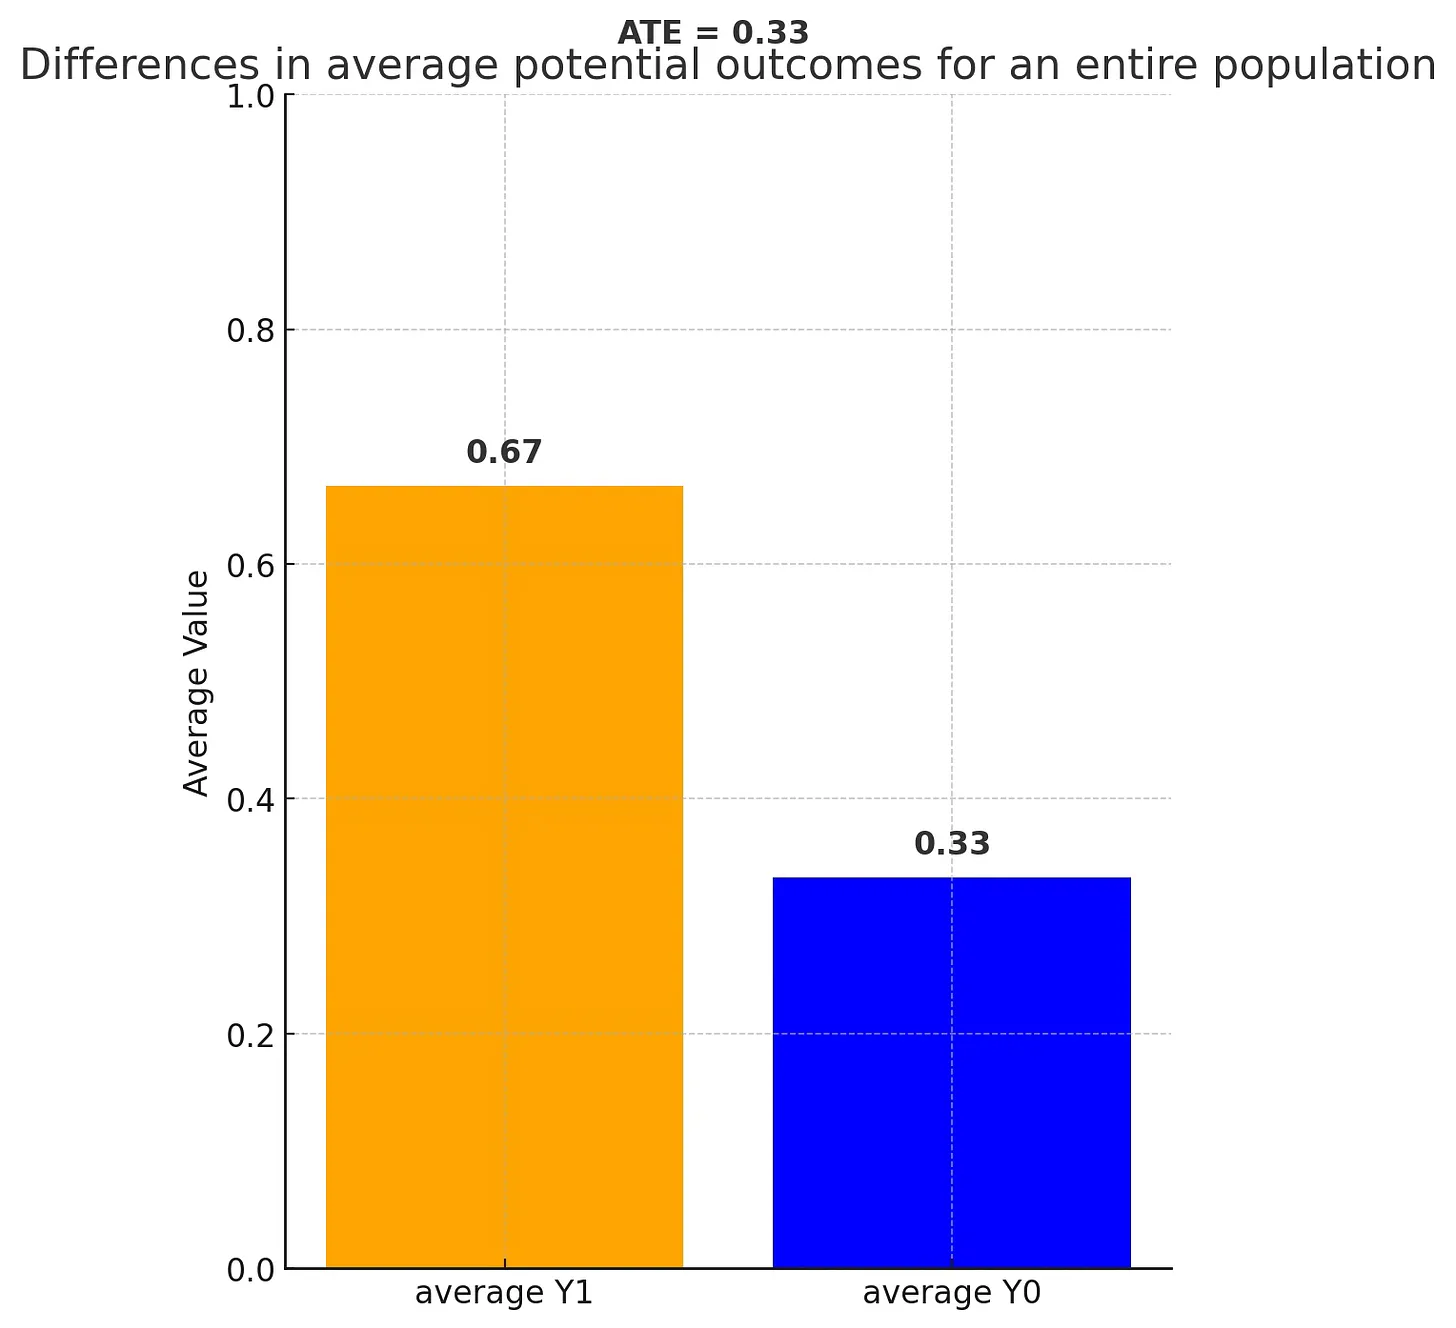
\includegraphics[height=0.8\textheight]{./lecture_includes/step1_y1y0}
\end{figure}


\end{frame}

\begin{frame}{Average Treatment Effect on the Treated}

\begin{figure}
    \centering
    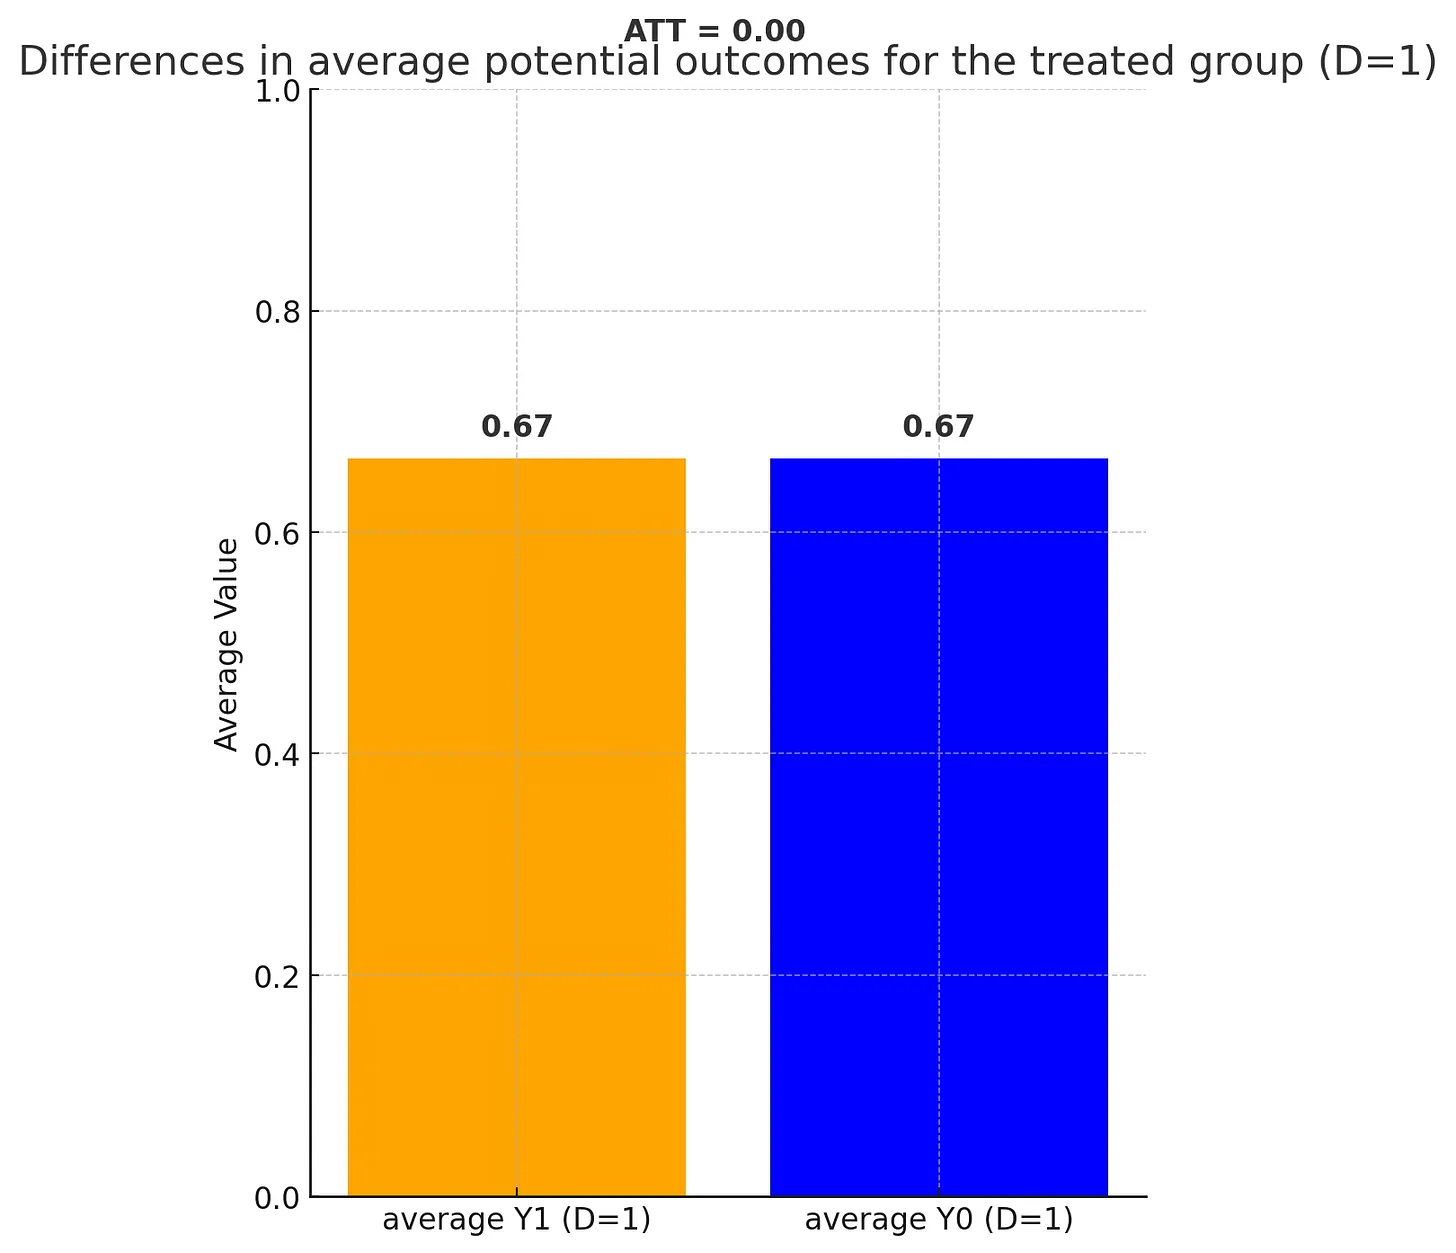
\includegraphics[height=0.8\textheight]{./lecture_includes/step1_att}
\end{figure}


\end{frame}



\begin{frame}{Which causal effect do you want?}

\begin{itemize}
\item We know diff-in-diff identifies the ATT not the ATE but there are still more than one ATT!
\item Solon, Haider and Wooldridge (2015), "What are we weighting for?"
\item Why you weight in surveys and why you weight in causal inference are different
	\begin{itemize}
	\item Survey weights are to make estimates nationally representative
	\item Population weighting in causal inference is because you want a different parameter
	\end{itemize}
\item How do we interpret adjustments made with population weights versus not?
\end{itemize}

\end{frame}




\begin{frame}{Different Levels of Aggregation, Different Weights}

\begin{table}[htbp]\centering
\footnotesize
\begin{tabular}{lcccc}
\toprule
\textbf{Individuals} & \textbf{Y\textsubscript{1}} & \textbf{Y\textsubscript{0}} & \textbf{$\delta$} & \textbf{County} \\
\midrule
Alan    & 1 & 0 & 1  & \cellcolor{yellow!30}1 \\
Betty   & 1 & 1 & 0  & \cellcolor{yellow!30}1 \\
Chad    & 1 & 1 & 0  & \cellcolor{yellow!30}1 \\
Daniel  & 0 & 0 & 0  & \cellcolor{yellow!30}1 \\
Edith   & 1 & 0 & 1  & \cellcolor{yellow!30}1 \\
Frank   & 1 & 0 & 1  & \cellcolor{yellow!30}1 \\
George  & 0 & 0 & 0  & \cellcolor{yellow!30}1 \\
Hank    & 1 & 0 & 1  & \cellcolor{yellow!30}1 \\
Ida     & 0 & 1 & -1 & \cellcolor{green!20}2 \\
Janet   & 0 & 1 & -1 & \cellcolor{green!20}2 \\
\midrule
\textbf{County} & & & \textbf{ATE\textsubscript{c}} & \\
\cellcolor{yellow!30}1 & & & \cellcolor{yellow!30}0.5 & \\
\cellcolor{green!20}2 & & & \cellcolor{green!20}-1 & \\
\midrule
\multicolumn{3}{l}{ATE for average county} & -0.25 & \\
\multicolumn{3}{l}{ATE for average person}   & 0.2 & \\
\bottomrule
\end{tabular}
\end{table}


\end{frame}

\begin{frame}{Weighting formula}

\begin{itemize}
\item What if you have city or county level data but you want the ATE for the average person?
\item Then that is when you weight by population -- because you want to know the effect for the \emph{average person}
\end{itemize}

\begin{equation}
ATE_{\text{people}} = \frac{\sum_c ATE_c \cdot N_c}{\sum_c N_c}
\end{equation}

\begin{eqnarray*}
ATE_p &=& \frac{(0.5 \times 8) + (-1 \times 2)}{8 + 2} \\
      &=& \frac{4 - 2}{10} \\
      &=& 0.2
\end{eqnarray*}

\end{frame}




\begin{frame}{Different Levels of Aggregation, Different Weights}


\begin{itemize}
\item Heterogenous treatment effects is causing this, but so is weighting
\item Consider Texas
	\begin{itemize}
	\item Texas has 31 million residents
	\item Texas 254 counties
	\end{itemize}
\item Where do they live?
	\begin{itemize}
	\item 13 million live in Harris, Dallas, Fort Worth, San Antonio and Austin, or rather 41\%
	\end{itemize}
\item What if concealed carry increases firearm deaths in cities, but reduces them in counties, because of sorting by treatment effects?
\end{itemize}

\end{frame}

\begin{frame}{Simulation}

\begin{itemize}
\item Assume a state with 30 million people and 254 counties
	\begin{itemize}
	\item 15 million live in 5 counties
	\item 15 million live equally spread in the other 249 counties (around 60,000 each)
	\end{itemize}
\item Assume that $\delta_i$ varies, sometimes positive and sometimes negative and $E[Y^1 - Y^0] = 2$
\end{itemize}

\end{frame}

\begin{frame}{Selection into Counties is Random}

\begin{itemize}
\item People choose where to live in Texas, but the mechanism by which they do so will have implications for our datasets
\item What if they sort into counties (i.e., where they live) by lottery
\item Every county will therefore have the same distribution of $Y^1$ and $Y^0$
\item Every county will have an ATE of $2$
\end{itemize}

\end{frame}



\begin{frame}{Average County ATE and Overall ATE Are the Same }

\begin{figure}
    \centering
    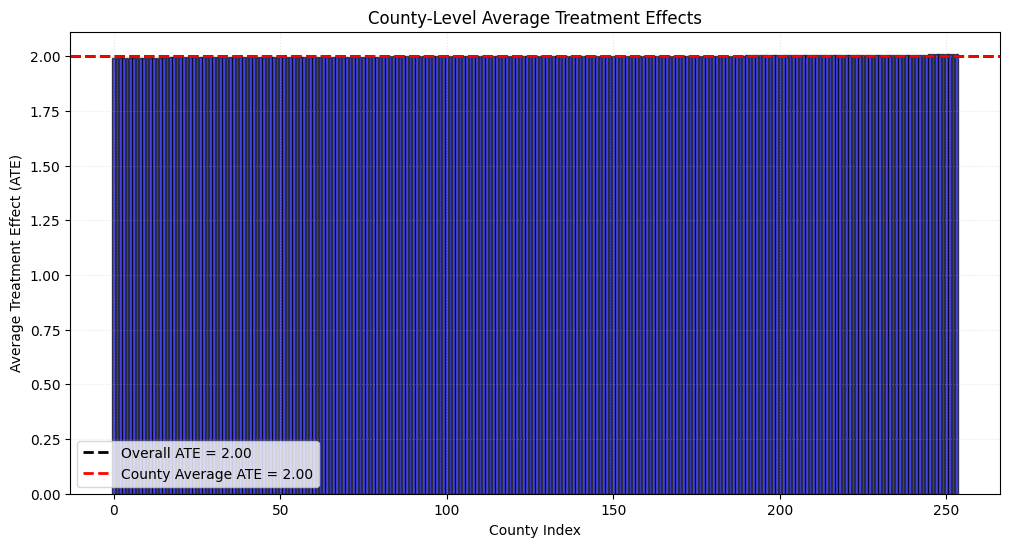
\includegraphics[height=0.7\textheight]{./lecture_includes/tiebout_roy1}
\end{figure}

\end{frame}

\begin{frame}{Selection into Counties is Based on Potential Outcomes}

\begin{itemize}
\item Now assume that people sort into five largest counties have the highest treatment effects ($\delta_i$)
\item Thus the five largest counties are those people for whom concealed carry guns law cause homicides
\item Remaining 249 small counties, in decreasing order, get residents with lower treatment effects (i.e., for whom concealed carry reduces murders)
\end{itemize}

\end{frame}

\begin{frame}{Average County ATE and Overall ATE Differ }

\begin{figure}
    \centering
    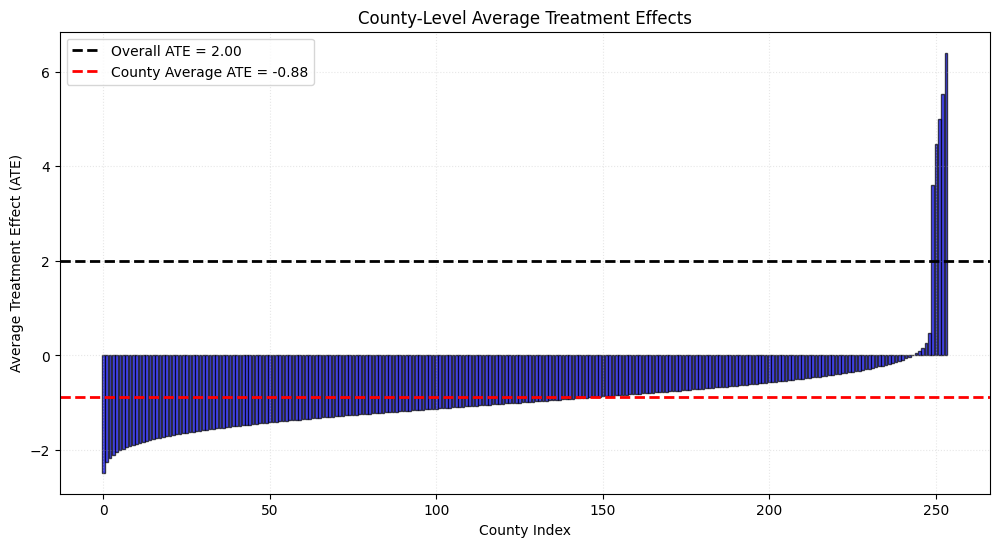
\includegraphics[height=0.7\textheight]{./lecture_includes/tiebout_roy2}
\end{figure}

\end{frame}




\begin{frame}{Both Are Valid, But Not Necessarily Your Research Question}

\begin{itemize}
\item Do you want to know the ATT for the \emph{average person} or the \emph{average county}?
	\begin{itemize}
	\item It depends on what your study is about, and it will absolutely matter for policy relevance, estimation and interpretability
	\item If it about the average person, then you want the overall ATT (i.e., the first case)
	\item If it is about the average county, then you want the county average ATT (i.e., the second case)
	\end{itemize}
\item Since you're averaging over \emph{units} in \emph{data}, it's imperative you make a decision early on as it changes what you decide
\item You can always use population weights but in causal inference, you ask what your target parameter is, and then decide your weights
\end{itemize}

\end{frame}

\begin{frame}{Choosing your ATT parameter}

\begin{itemize}

\item As a rule, imagine who your audience is, and what you both agree the policy levers are
\item In the US, local municipalities have a lot of discretion to pass their own laws -- even in areas where you might think it was impossible to imagine like the decriminalization of drugs
\item It may be \emph{local} policy makers want to know the causal effect on \emph{local communities} in which case you \textbf{don't weight}
\item If you are ever unsure, \emph{do both to avoid cherry picking} but \emph{be clear}.

\end{itemize}

\end{frame}




\end{document}
